\documentclass[12pt,a4paper]{article}
\usepackage[provide=*,italian]{babel}
\usepackage{fontspec}
\setmainfont{NimbusSans-Regular.otf}[BoldFont=NimbusSans-Bold.otf,ItalicFont=NimbusSans-Italic.otf,BoldItalicFont=NimbusSans-BoldItalic.otf]
\usepackage[a4paper,margin=2.5cm,headheight=15pt]{geometry}
\usepackage{setspace}
\setstretch{1.5}
\setlength{\parindent}{0pt}
\setlength{\parskip}{5pt}
\usepackage{graphicx,longtable,booktabs,array,calc,pdflscape}
\usepackage{amsmath,amssymb,xcolor}
\providecommand{\hl}[1]{#1}
\providecommand{\ul}[1]{#1}
\usepackage{hyperref}
\hypersetup{hidelinks,pdftitle={TESI - Asia Rimondi},pdfauthor={Asia Rimondi}}
\usepackage{titlesec}
\titleformat{\section}{\normalfont\bfseries\fontsize{16}{20}\selectfont}{}{0pt}{}
\titleformat{\subsection}{\normalfont\bfseries\fontsize{14}{18}\selectfont}{}{0pt}{}
\titleformat{\subsubsection}{\normalfont\bfseries\fontsize{12}{16}\selectfont}{}{0pt}{}
\titlespacing*{\section}{0pt}{0pt}{13pt}
\titlespacing*{\subsection}{0pt}{12pt}{8pt}
\titlespacing*{\subsubsection}{0pt}{10pt}{6pt}
\setcounter{secnumdepth}{-2}
\pagestyle{empty}
\setlength{\emergencystretch}{3em}
\providecommand{\tightlist}{\setlength{\itemsep}{0pt}\setlength{\parskip}{0pt}}
\makeatletter
\def\maxwidth{\ifdim\Gin@nat@width>\linewidth\linewidth\else\Gin@nat@width\fi}
\def\maxheight{\ifdim\Gin@nat@height>\textheight\textheight\else\Gin@nat@height\fi}
\makeatother
\setkeys{Gin}{width=\maxwidth,height=\maxheight,keepaspectratio}
\urlstyle{same}
\begin{document}
\begin{titlepage}
\begin{center}
\setstretch{1}
\vspace*{-0.7cm}

\includegraphics[width=5.0cm]{immagini/image1.png}\\[.65cm]
{\bfseries\fontsize{12}{15}\selectfont DIPARTIMENTO DI SCIENZE MEDICHE E CHIRURGICHE - DIMEC\par}
\vspace{.9cm}
{\bfseries\fontsize{14}{18}\selectfont CORSO DI LAUREA IN\\
TECNICHE DI RADIOLOGIA MEDICA, PER IMMAGINI E RADIOTERAPIA\par}
\vspace{.75cm}
{\bfseries\fontsize{21}{29}\selectfont Utilizzo del fusion imaging ecocardiografico-fluoroscopico nelle procedure transcatetere sulle valvole atrioventricolari: una revisione sistematica della letteratura\par}
\vspace{.75cm}
{\bfseries\fontsize{12}{16}\selectfont Tesi di laurea in Tecniche di Imaging Angiografiche\par}
\end{center}
\vspace{.75cm}
\noindent\begin{minipage}[t]{.52\textwidth}\bfseries\fontsize{14}{19}\selectfont
Relatore:\\Prof. Michele Gregori\\[.4cm]
Correlatrice:\\Dott. Giulia Carpanelli
\end{minipage}\hfill\begin{minipage}[t]{.27\textwidth}\bfseries\fontsize{14}{19}\selectfont
Presentata da:\\Asia Rimondi
\end{minipage}
\vfill
\noindent\rule{\textwidth}{.8pt}
\begin{center}\bfseries\fontsize{12}{16}\selectfont
I Sessione, Ottobre 2026\\Anno Accademico 2025/2026
\end{center}
\end{titlepage}
\setcounter{page}{2}
\clearpage
\begingroup\fontsize{9.5}{11}\selectfont\setstretch{1}\setlength{\parskip}{0pt}
\hypertarget{indice}{%
\section*{Indice}\label{indice}}

\protect\hyperlink{abstract}{\textbf{Abstract}}\dotfill\pageref{abstract}

\protect\hyperlink{introduzione}{\textbf{Introduzione}}\dotfill\pageref{introduzione}

\protect\hyperlink{anatomia-fisiopatologia-e-trattamento-transcatetere-delle-valvole-atrioventricolari}{\textbf{1. Anatomia, fisiopatologia e trattamento transcatetere delle valvole atrioventricolari}}\dotfill\pageref{anatomia-fisiopatologia-e-trattamento-transcatetere-delle-valvole-atrioventricolari}

\begingroup\leftskip=1cm\relax
\protect\hyperlink{anatomia-della-valvola-mitrale-e-dellapparato-sottovalvolare}{1.1 Anatomia della valvola mitrale e dell'apparato sottovalvolare}\dotfill\pageref{anatomia-della-valvola-mitrale-e-dellapparato-sottovalvolare}

\protect\hyperlink{insufficienza-mitralica}{1.2 Insufficienza mitralica}\dotfill\pageref{insufficienza-mitralica}

\protect\hyperlink{anatomia-della-valvola-tricuspide-e-dellapparato-sottovalvolare}{1.3 Anatomia della valvola tricuspide e dell'apparato sottovalvolare}\dotfill\pageref{anatomia-della-valvola-tricuspide-e-dellapparato-sottovalvolare}

\protect\hyperlink{insufficienza-tricuspidale}{1.4 Insufficienza tricuspidale}\dotfill\pageref{insufficienza-tricuspidale}

\protect\hyperlink{procedure-transcatetere-di-riparazione-e-sostituzione-delle-valvole-atrioventricolari}{1.5 Procedure transcatetere di riparazione e sostituzione delle valvole atrioventricolari}\dotfill\pageref{procedure-transcatetere-di-riparazione-e-sostituzione-delle-valvole-atrioventricolari}

\protect\hyperlink{sistema-mitraclip-e-pascal-per-la-riparazione-transcatetere-edge-to-edge-della-valvola-mitrale}{1.5.1 Sistema MitraClip e PASCAL per la riparazione transcatetere edge-to-edge della valvola mitrale}\dotfill\pageref{sistema-mitraclip-e-pascal-per-la-riparazione-transcatetere-edge-to-edge-della-valvola-mitrale}

\protect\hyperlink{sistema-triclip-e-pascal-per-la-riparazione-transcatetere-edge-to-edge-della-valvola-tricuspide}{1.5.2 Sistema TriClip e PASCAL per la riparazione transcatetere edge-to-edge della valvola tricuspide}\dotfill\pageref{sistema-triclip-e-pascal-per-la-riparazione-transcatetere-edge-to-edge-della-valvola-tricuspide}

\protect\hyperlink{sistema-evoque-per-la-sostituzione-transcatetere-della-valvola-tricuspide-e-mitrale}{1.5.3 Sistema EVOQUE per la sostituzione transcatetere della valvola tricuspide e mitrale}\dotfill\pageref{sistema-evoque-per-la-sostituzione-transcatetere-della-valvola-tricuspide-e-mitrale}

\protect\hyperlink{sistema-intrepid-per-la-sostituzione-transcatetere-della-valvola-mitrale}{1.5.4 Sistema Intrepid per la sostituzione transcatetere della valvola mitrale}\dotfill\pageref{sistema-intrepid-per-la-sostituzione-transcatetere-della-valvola-mitrale}
\endgroup

\protect\hyperlink{fusion-imaging-ecocardiografico-fluoroscopico}{\textbf{2. Fusion imaging ecocardiografico-fluoroscopico}}\dotfill\pageref{fusion-imaging-ecocardiografico-fluoroscopico}

\begingroup\leftskip=1cm\relax
\protect\hyperlink{principi-generali-del-fusion-imaging}{2.1 Principi generali del fusion imaging}\dotfill\pageref{principi-generali-del-fusion-imaging}

\protect\hyperlink{riparazione-transcatetere-edge-to-edge-della-valvola-mitrale}{2.2 Riparazione transcatetere edge-to-edge della valvola mitrale}\dotfill\pageref{riparazione-transcatetere-edge-to-edge-della-valvola-mitrale}

\protect\hyperlink{puntura-transettale-e-marker}{2.2.1 Puntura transettale e marker}\dotfill\pageref{puntura-transettale-e-marker}

\protect\hyperlink{navigazione-dei-cateteri-e-dei-sistemi-di-rilascio}{2.2.2 Navigazione dei cateteri e dei sistemi di rilascio}\dotfill\pageref{navigazione-dei-cateteri-e-dei-sistemi-di-rilascio}

\protect\hyperlink{allineamento-e-posizionamento-del-dispositivo}{2.2.3 Allineamento e posizionamento del dispositivo}\dotfill\pageref{allineamento-e-posizionamento-del-dispositivo}

\protect\hyperlink{cattura-dei-lembi-rilascio-e-controllo-finale}{2.2.4 Cattura dei lembi, rilascio e controllo finale}\dotfill\pageref{cattura-dei-lembi-rilascio-e-controllo-finale}

\protect\hyperlink{ruolo-del-tsrm}{2.3 Ruolo del TSRM}\dotfill\pageref{ruolo-del-tsrm}
\endgroup

\protect\hyperlink{materiali-e-metodi-della-revisione-sistematica}{\textbf{3. Materiali e metodi della revisione sistematica}}\dotfill\pageref{materiali-e-metodi-della-revisione-sistematica}

\begingroup\leftskip=1cm\relax
\protect\hyperlink{ricerca-bibliografica}{3.1 Ricerca bibliografica}\dotfill\pageref{ricerca-bibliografica}

\protect\hyperlink{metodo-di-conduzione-della-revisione-sistematica}{3.2 Metodo di conduzione della revisione sistematica}\dotfill\pageref{metodo-di-conduzione-della-revisione-sistematica}

\protect\hyperlink{criteri-di-eleggibilituxe0-inclusione-ed-esclusione}{3.2.1 Criteri di eleggibilità, inclusione ed esclusione}\dotfill\pageref{criteri-di-eleggibilituxe0-inclusione-ed-esclusione}

\protect\hyperlink{estrazione-dati}{3.2.2 Estrazione dati}\dotfill\pageref{estrazione-dati}
\endgroup

\protect\hyperlink{risultati}{\textbf{4. Risultati}}\dotfill\pageref{risultati}

\begingroup\leftskip=1cm\relax
\protect\hyperlink{selezione-degli-articoli}{4.1 Selezione degli articoli}\dotfill\pageref{selezione-degli-articoli}

\protect\hyperlink{studi-inclusi}{4.2 Studi inclusi}\dotfill\pageref{studi-inclusi}

\protect\hyperlink{valutazione-del-rischio-di-bias---robins-i-risk-of-bias-in-non-randomized-studies-of-interventions}{4.3 Valutazione del rischio di bias - ROBINS-I (Risk Of Bias In Non-randomized Studies of Interventions)}\dotfill\pageref{valutazione-del-rischio-di-bias---robins-i-risk-of-bias-in-non-randomized-studies-of-interventions}
\endgroup

\protect\hyperlink{discussione}{\textbf{5. Discussione}}\dotfill\pageref{discussione}

\begingroup\leftskip=1cm\relax
\protect\hyperlink{effetto-del-fusion-imaging-sui-tempi-procedurali}{5.1 Effetto del fusion imaging sui tempi procedurali}\dotfill\pageref{effetto-del-fusion-imaging-sui-tempi-procedurali}

\protect\hyperlink{effetto-del-fusion-imaging-sulla-fluoroscopia-e-sullesposizione-radiologica}{5.2 Effetto del fusion imaging sulla fluoroscopia e sull'esposizione radiologica}\dotfill\pageref{effetto-del-fusion-imaging-sulla-fluoroscopia-e-sullesposizione-radiologica}

\protect\hyperlink{limiti}{5.3 Limiti}\dotfill\pageref{limiti}
\endgroup

\protect\hyperlink{conclusioni}{\textbf{6. Conclusioni}}\dotfill\pageref{conclusioni}

\protect\hyperlink{bibliografia}{\textbf{7. Bibliografia}}\dotfill\pageref{bibliografia}

\protect\hyperlink{ringraziamenti}{\textbf{8. Ringraziamenti}}\dotfill\pageref{ringraziamenti}

\endgroup
\clearpage
\hypertarget{abstract}{%
\section*{Abstract}\label{abstract}}

La presente revisione sistematica valuta i potenziali benefici del fusion imaging ecocardiografico-fluoroscopico durante le procedure transcatetere sulle valvole atrioventricolari.

La ricerca bibliografica è stata condotta su PubMed, Scopus, Web of Science e Health \& Medical Collection (2016-2026), secondo le linee guida PRISMA 2020. Il quesito valuta se l'impiego del fusion imaging, rispetto alla guida convenzionale basata sulla visualizzazione separata delle immagini, sia associato a una riduzione dell'esposizione alle radiazioni ionizzanti, della durata procedurale e del tempo di fluoroscopia, nonché a un miglioramento del successo procedurale e della sicurezza.

Sono stati considerati eleggibili studi clinici originali su pazienti adulti sottoposti a procedure transcatetere sulle valvole atrioventricolari. Inoltre era necessario che confrontassero un gruppo guidato mediante fusion imaging con uno di controllo utilizzando la guida di imaging convenzionale.

Duplicati e screening sono stati gestiti con Rayyan; il rischio di bias è stato valutato con ROBINS-I.

Sono stati inclusi tre studi osservazionali retrospettivi con disegno prima-dopo, tutti comprendenti pazienti sottoposti a MitraClip. Due studi hanno evidenziato una riduzione statisticamente significativa del tempo fino al completamento della puntura transettale: 4,72 minuti (Afzal 2017; p = 0,006) e 9,1 minuti (Afzal 2020; p \textless{} 0,001).

Melillo (2021) ha rilevato una riduzione di 11 minuti (p = 0,003) e un maggiore successo procedurale. Non sono emerse differenze significative nella durata procedurale totale, negli indicatori dosimetrici DAP/KAP e nelle complicanze.

Il numero limitato di studi, il disegno osservazionale retrospettivo e i risultati non uniformi non consentono di trarre conclusioni definitive sui benefici del fusion imaging; sono pertanto necessari ulteriori studi comparativi.

\clearpage
\hypertarget{introduzione}{%
\section*{\texorpdfstring{Introduzione }{Introduzione }}\label{introduzione}}

Le procedure transcatetere sulle valvole atrioventricolari vengono eseguite mediante la guida combinata dell'ecocardiografia e della fluoroscopia, due metodiche che forniscono informazioni complementari durante le diverse fasi dell'intervento. L'ecocardiografia permette di visualizzare l'anatomia cardiaca e i tessuti molli, mentre la fluoroscopia consente di seguire la navigazione e il posizionamento dei cateteri e dei dispositivi. {[}1{]}

L'impiego della fluoroscopia comporta tuttavia l'esposizione del paziente e degli operatori alle radiazioni ionizzanti e rende quindi rilevante la valutazione di strategie volte a modulare i parametri esposimetrici. Questo aspetto assume particolare interesse per il tecnico sanitario di radiologia medica (TSRM), che contribuisce all'ottimizzazione dell'impiego dell'imaging radiologico durante la procedura.

Nella guida convenzionale, le immagini ecocardiografiche e fluoroscopiche vengono visualizzate separatamente. Questa modalità richiede agli operatori di integrare mentalmente le informazioni fornite dalle due metodiche durante la navigazione e il posizionamento dei dispositivi. Per facilitare l'integrazione di queste informazioni, negli ultimi anni sono stati introdotti nella pratica clinica sistemi di fusion imaging ecocardiografico-fluoroscopico, in grado di co-registrare le due metodiche e di sovrapporre le informazioni ecocardiografiche sulle immagini fluoroscopiche. {[}1, 2{]}

Da questo presupposto nasce il quesito della presente revisione sistematica, finalizzata a valutare i potenziali benefici del fusion imaging ecocardiografico-fluoroscopico nelle procedure transcatetere sulle valvole mitrale e tricuspide. In particolare, sono stati analizzati i possibili effetti della tecnologia sul tempo procedurale, sul tempo di fluoroscopia, sull'esposizione alle radiazioni ionizzanti, sul successo procedurale e sulla sicurezza.

Durante la revisione linguistica, la riformulazione e l'impostazione della struttura della tesi sono stati usati modelli linguistici di grandi dimensioni (LLM), quali ChatGPT e Gemini. I contenuti scientifici, le fonti e la revisione finale sono stati verificati e validati dall'autrice insieme al relatore e alla correlatrice.

\clearpage
\hypertarget{anatomia-fisiopatologia-e-trattamento-transcatetere-delle-valvole-atrioventricolari}{%
\section*{1. Anatomia, fisiopatologia e trattamento transcatetere delle valvole atrioventricolari}\label{anatomia-fisiopatologia-e-trattamento-transcatetere-delle-valvole-atrioventricolari}}

\hypertarget{anatomia-della-valvola-mitrale-e-dellapparato-sottovalvolare}{%
\subsection*{1.1 Anatomia della valvola mitrale e dell'apparato sottovalvolare}\label{anatomia-della-valvola-mitrale-e-dellapparato-sottovalvolare}}

La valvola mitrale (o atrioventricolare sinistra) è una struttura cardiaca di tessuto connettivo situata tra l'atrio e il ventricolo sinistro. Essa fa parte di un complesso apparato anatomico le cui componenti interagiscono in modo armonico per evitare il reflusso sanguigno in atrio durante la sistole ventricolare. {[}3, 4{]}

L'apparato mitralico è composto da quattro elementi principali: l'anulus fibroso, i due lembi valvolari, le corde tendinee e i muscoli papillari.

L'anulus fibroso presenta una conformazione a sella e costituisce una porzione dello scheletro fibroso cardiaco, offrendo supporto strutturale e conferendo stabilità all'intero complesso valvolare. {[}5{]}

I due lembi (o cuspidi) valvolari si distinguono in anteriore, rivolto verso l'orifizio aortico e posizionato tra due trigoni fibrosi {[}5{]}, e posteriore. Si aprono durante la diastole e si chiudono in sistole. Entrambi i lembi sono suddivisi in tre settori o scallop, numerati da 1 a 3 in senso latero-mediale, assumendo l'auricola sinistra come punto di riferimento per il lato laterale (A1, A2, A3 per il lembo anteriore e P1, P2, P3 per il lembo posteriore). I punti di giunzione tra i due lembi prendono il nome di commissure valvolari (antero-laterale e postero-mediale).

L'apparato sottovalvolare è formato dalle corde tendinee e dai muscoli papillari (supero-posteriore o anteriore e inferiore o posteriore). {[}3{]}

Le corde tendinee ancorano sia i margini liberi sia la superficie ventricolare delle cuspidi all'apice dei muscoli papillari. Durante la sistole ventricolare, la contrazione sincrona dei muscoli papillari mette in tensione le corde tendinee, bilanciando la spinta della pressione intraventricolare; questo meccanismo previene il prolasso dei lembi in atrio e favorisce una corretta coaptazione valvolare. {[}4{]}

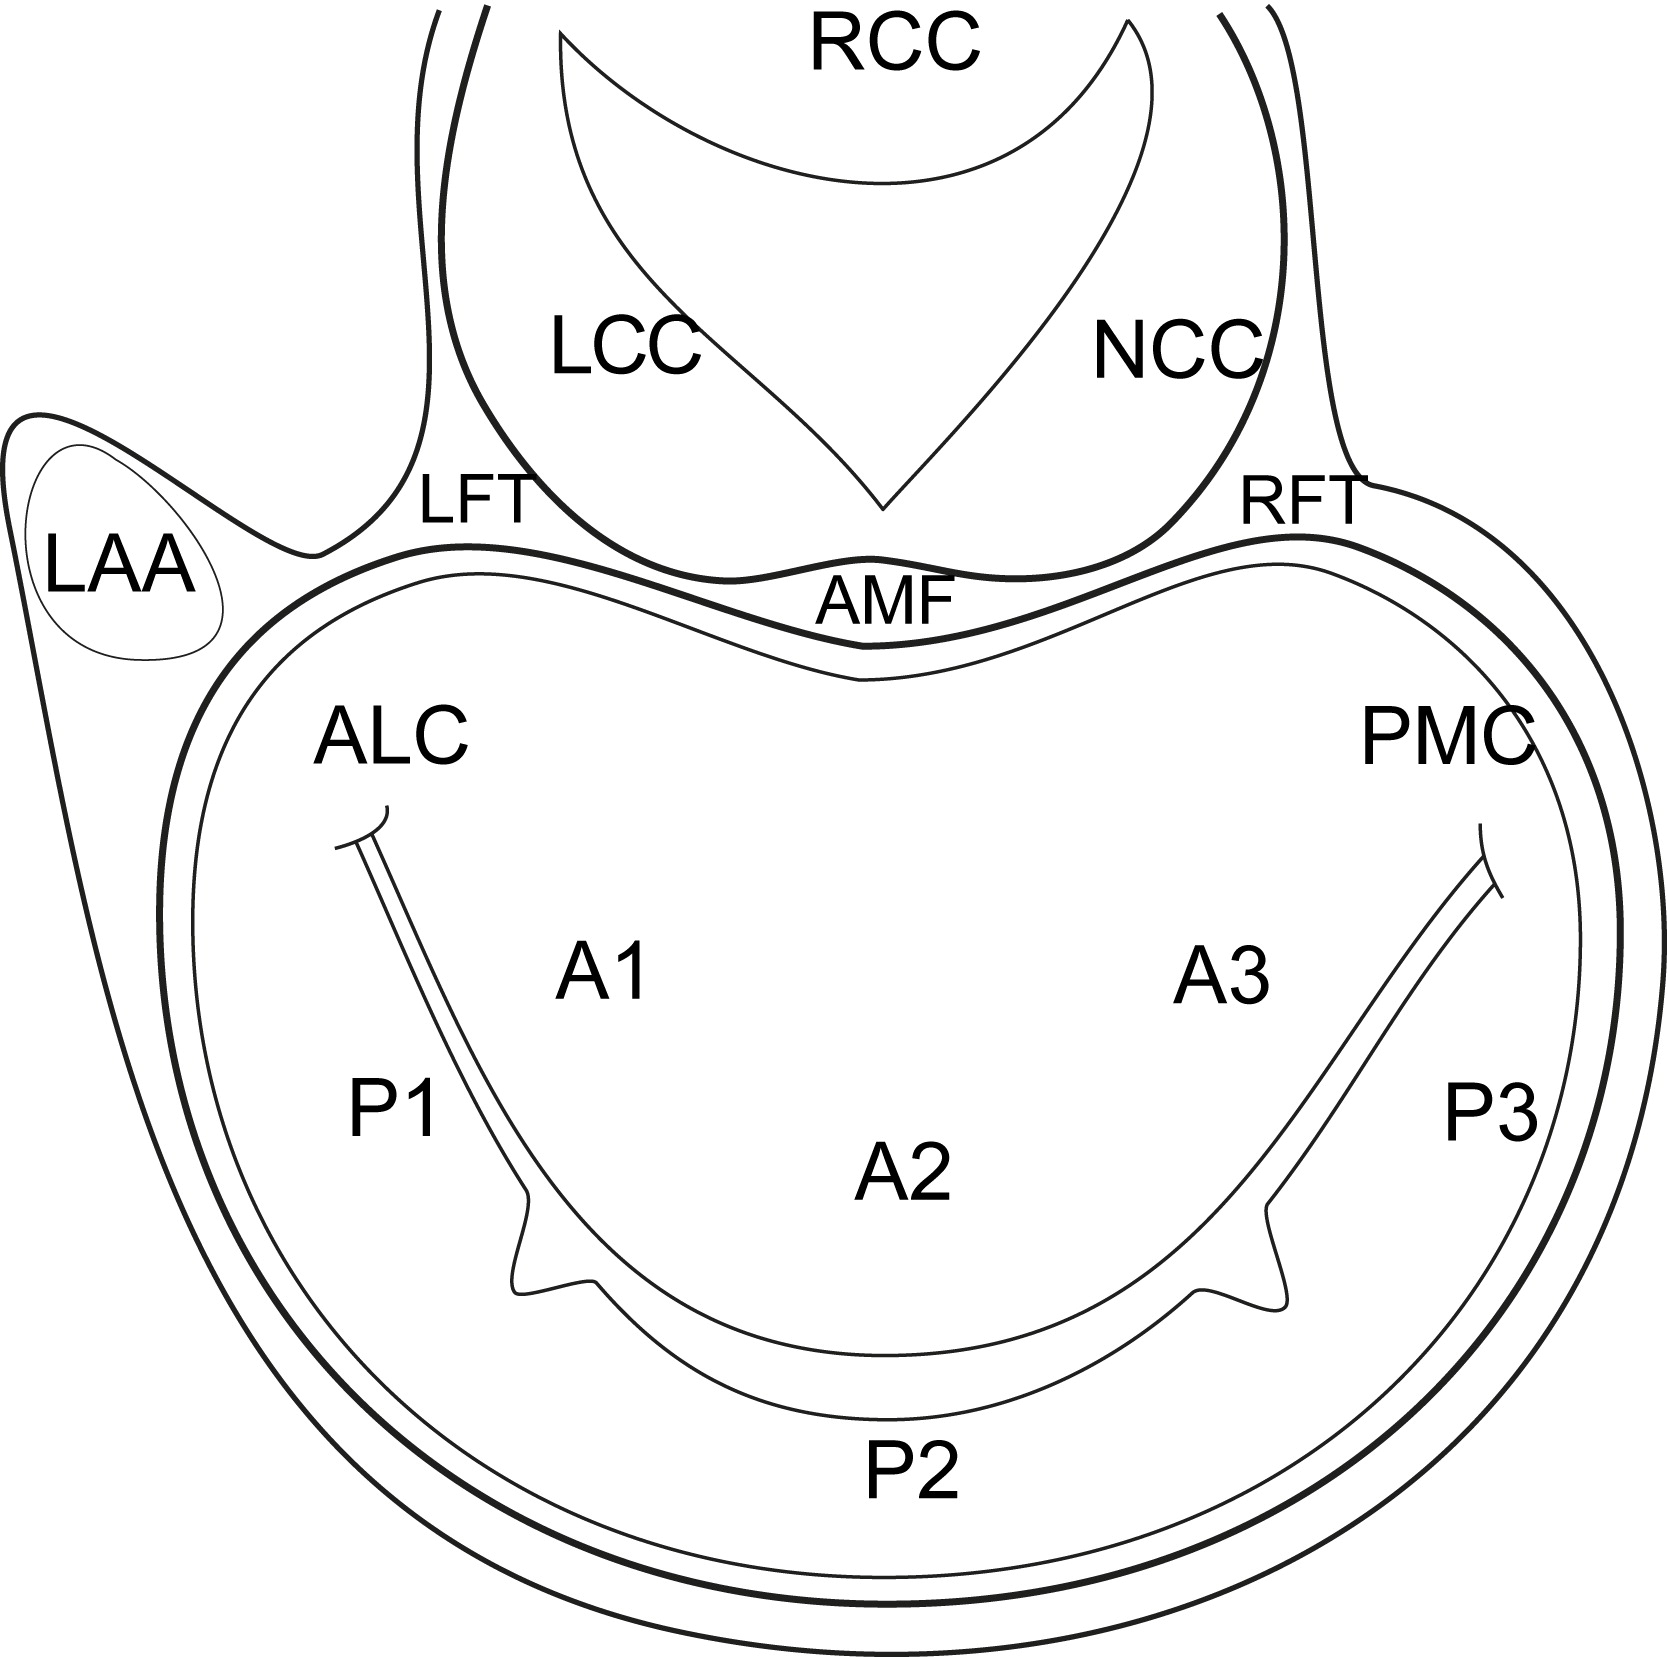
\includegraphics[width=2.57362in,height=2.56262in]{immagini/image3.jpg}

\textbf{Figura 1. Schema anatomico della valvola mitrale vista dall'atrio sinistro, con i segmenti A1--A3 del lembo anteriore e P1--P3 del lembo posteriore. Riprodotta da Salcedo et al. {[}31{]}, fig. 5. © 2009 American Society of Echocardiography, con autorizzazione tramite Elsevier.}\footnote{Reprinted from Journal of the American Society of Echocardiography, Vol. 22, Salcedo EE, Quaife RA, Seres T, Carroll JD, ``A framework for systematic characterization of the mitral valve by real-time three-dimensional transesophageal echocardiography'', pp. 1087--1099, Copyright (2009), with permission from the American Society of Echocardiography.}

\hypertarget{insufficienza-mitralica}{%
\subsection*{1.2 Insufficienza mitralica}\label{insufficienza-mitralica}}

L'insufficienza mitralica è una patologia valvolare caratterizzata dall\textquotesingle incompleta chiusura della valvola mitrale durante la sistole ventricolare. Tale alterazione provoca il rigurgito di sangue dal ventricolo sinistro all'atrio sinistro, determinando un sovraccarico di volume delle cavità cardiache sinistre che può portare progressivamente a rimodellamento ventricolare, riduzione della gittata cardiaca, aritmie, endocarditi, insufficienza cardiaca, edema polmonare acuto e, nei casi più avanzati, morte. {[}6, 7{]}

In Europa, l'insufficienza mitralica (IM) rappresenta la seconda valvulopatia più frequente e per cui si richiede un trattamento. Una recente revisione sistematica con meta-analisi ha stimato una prevalenza di IM moderata-grave nella popolazione generale pari allo 0,60\% (IC 95\% 0,34--0,92), corrispondente a circa 6 persone ogni 1000. {[}32{]}

Una corretta classificazione è fondamentale, poiché l'approccio terapeutico varia in funzione del meccanismo sottostante, distinguendo tra forme primarie e secondarie. {[}8{]}

L'IM si può classificare secondo diversi criteri che possono riguardare la modalità di insorgenza (acuta o cronica), l'eziologia (primaria o secondaria), il grado di severità e il movimento dei lembi valvolari, secondo la classificazione funzionale di Carpentier. {[}6, 9{]}

L'IM acuta rappresenta un'emergenza cardiovascolare, associata a un'elevata mortalità e alla frequente necessità di un trattamento chirurgico urgente. Le principali cause comprendono l'endocardite infettiva, la rottura delle corde tendinee, la disfunzione o la rottura del muscolo papillare in seguito a infarto miocardico acuto e i traumi toracici. Dal punto di vista fisiopatologico, il rigurgito improvviso determina un rapido incremento della pressione nell'atrio sinistro, con conseguente congestione ed edema polmonare. Il trattamento iniziale prevede la stabilizzazione emodinamica mediante diuretici e vasodilatatori per ridurre il postcarico; nei pazienti instabili come terapia supportiva può essere utilizzato il contropulsatore aortico (Intra-Aortic Balloon Pump, IABP) in attesa del trattamento definitivo, generalmente chirurgico. {[}6{]}

L'IM cronica è inizialmente asintomatica e si suddivide a sua volta in primaria (o organica) e secondaria (o funzionale).

L'IM primaria può derivare da patologie degenerative o reumatiche ed è conseguente al danneggiamento di una o più componenti del complesso valvolare mitralico e, in questo caso, rappresenta l'evento iniziale che precede il rimodellamento del ventricolo sinistro. Tra le eziologie emergenti è stata descritta anche la cardiopatia da esposizione a radiazioni ionizzanti; inoltre, è frequente riscontrare pazienti con calcificazione dell'anulus mitralico. Quando indicato, il trattamento è preferibilmente rappresentato dalla riparazione della valvola mitrale; la sostituzione valvolare viene riservata ai casi in cui la riparazione non sia possibile. {[}6{]}

L'IM secondaria origina da una disfunzione ventricolare causata dal rimodellamento e dalla dilatazione del ventricolo sinistro. Sebbene la valvola mitrale e le sue componenti siano strutturalmente integre, tali alterazioni determinano una coaptazione incompleta dei lembi valvolari e, di conseguenza, il rigurgito. Alcuni pazienti possono inoltre presentare una dilatazione dell'atrio sinistro, spesso conseguente a una fibrillazione atriale cronica, che provoca la dilatazione dell'anulus mitralico e contribuisce all'insufficienza mitralica. {[}6{]}

La classificazione di Carpentier distingue l'IM in tre principali tipologie sulla base della funzionalità valvolare.

\begin{itemize}
\item
  \begin{quote}
  Tipo I: la motilità dei lembi valvolari risulta nella norma; il rigurgito è generalmente causato da una dilatazione dell'anulus mitralico oppure da una perforazione di uno dei due lembi.
  \end{quote}
\item
  \begin{quote}
  Tipo II: l'eccessiva mobilità dei lembi valvolari è dovuta al prolasso o al flail leaflet conseguente, ad esempio, all'allungamento o alla rottura delle corde tendinee.
  \end{quote}
\item
  \begin{quote}
  Tipo III: è caratterizzato da un movimento limitato dei lembi ed è suddiviso in due sottotipi:
  \end{quote}
\end{itemize}

\begin{quote}
- Tipo IIIa: la limitazione è presente in diastole, ed è tipicamente associata alla cardiopatia reumatica o ad altre patologie infiammatorie della valvola.

- Tipo IIIb: la limitazione interessa prevalentemente la sistole ed è generalmente secondaria al rimodellamento del ventricolo sinistro. {[}6, 9{]}
\end{quote}

L'IM viene inoltre classificata in base alla sua gravità mediante una valutazione ecocardiografica che si avvale del color Doppler, eseguita inizialmente con ecocardiografia transtoracica (TTE) e, quando indicato, con ecocardiografia transesofagea (TEE). La risonanza magnetica cardiaca (CMR) rappresenta un valido strumento complementare nella fase preprocedurale qualora i risultati precedenti risultino discordanti o sia necessario un esame più approfondito. In particolare, costituisce una metodica utile per la valutazione funzionale dei ventricoli e per la misurazione del volume e della frazione rigurgitante. {[}6, 9, 10, 11{]}

Prima di poter stabilire la gravità dell'IM, è necessario distinguere la forma primitiva, o organica, da quella secondaria, o funzionale, poiché l'interpretazione dei valori e alcune soglie di gravità possono variare in base all'eziologia. {[}8, 10{]}

Attraverso l'integrazione dei parametri qualitativi, semiquantitativi e quantitativi raccomandati dalle linee guida, il rigurgito mitralico viene classificato come lieve, moderato e severo. Le forme severe sono associate a un rischio maggiore di rimodellamento delle camere cardiache, progressione dello scompenso cardiaco, fibrillazione atriale e mortalità. {[}6, 9, 10{]}

I parametri qualitativi permettono di identificare visivamente il meccanismo e le alterazioni morfologiche responsabili del rigurgito, come la presenza di prolasso o flail di un lembo, e di valutare le caratteristiche e la direzione del jet rigurgitante. La vena contracta rappresenta invece un parametro semiquantitativo, mentre l'EROA (\emph{Effective Regurgitant Orifice Area}), il volume rigurgitante e la frazione rigurgitante costituiscono parametri quantitativi. {[}9{]}

La vena contracta corrisponde alla porzione più stretta del flusso rigurgitante, localizzata in corrispondenza o immediatamente a valle dell'orifizio. Una larghezza ≥ 7 mm, o ≥ 8 mm nella valutazione biplanare, è indicativa di un'IM severa. {[}9, 10{]}

L'EROA rappresenta l\textquotesingle area effettiva dell'orifizio attraverso il quale passa il flusso rigurgitante. Nell'IM primaria, un valore ≥ 0,40 cm\textsuperscript{2} è indicativo di severità. Nell'IM secondaria a causa della frequente conformazione ellittica dell'orifizio un'EROA ≥ 0,30 cm\textsuperscript{2} può essere compatibile con un rigurgito severo. {[}8, 10{]}

Un volume rigurgitante ≥ 60 ml è indicativo di IM severa, sebbene nell'IM secondaria possa assumere rilevanza anche un valore ≥ 45 ml. {[}8, 10{]}

Infine, una frazione rigurgitante ≥ 50\% rappresenta un ulteriore criterio quantitativo di severità {[}7, 9, 10{]}. Questi parametri non devono essere considerati isolatamente, ma integrati con gli altri reperti ecocardiografici e con il contesto clinico ed emodinamico.

\hypertarget{anatomia-della-valvola-tricuspide-e-dellapparato-sottovalvolare}{%
\subsection*{1.3 Anatomia della valvola tricuspide e dell'apparato sottovalvolare}\label{anatomia-della-valvola-tricuspide-e-dellapparato-sottovalvolare}}

La valvola tricuspide, costituita prevalentemente da tessuto connettivo, è posta tra l'atrio destro e il ventricolo destro e impedisce il reflusso del sangue dal ventricolo all'atrio durante la sistole. {[}12{]}

L'apparato valvolare comprende quattro componenti principali: l'anulus valvolare, i lembi, le corde tendinee e i muscoli papillari.

L'anulus fibroso presenta una conformazione a forma di D, con il lato settale relativamente rettilineo.

Normalmente, la valvola tricuspide viene descritta come costituita da tre lembi di differenti dimensioni, sebbene siano frequenti varianti anatomiche riguardanti il loro numero e la loro morfologia. In base alla loro disposizione spaziale, i lembi sono denominati anteriore, posteriore e settale. Il lembo anteriore, generalmente il più grande e il più mobile, è rivolto verso la parete anteriore del ventricolo destro e il tratto di efflusso ventricolare. Il lembo posteriore è solitamente più corto e può presentare diversi scallop, mentre il lembo settale è posto in prossimità del setto interventricolare, presenta una mobilità più limitata ed è collegato al setto mediante corde tendinee corte. {[}12{]}

L'ostio del seno coronarico è localizzato nell'atrio destro, in prossimità della commissura posterosettale, mentre la commissura anterosettale è adiacente al seno non coronarico di Valsalva. {[}12{]}

I muscoli papillari e le corde tendinee fanno parte del complesso sottovalvolare.

Generalmente sono presenti due muscoli papillari principali: il muscolo papillare anteriore, più grande, e quello posteriore, che può presentare una conformazione biforcuta o triforcuta. Può inoltre essere presente un muscolo papillare settale, generalmente di piccole dimensioni e talvolta assente. {[}12{]}

I muscoli papillari sono collegati ai lembi valvolari mediante le corde tendinee, costituite prevalentemente da collagene ed elastina e rivestite da cellule endoteliali. Possono inoltre essere presenti corde false che, pur non inserendosi sui lembi valvolari, possono collegare tra loro due muscoli papillari oppure unire i muscoli alla parete ventricolare. {[}12{]}

\hypertarget{insufficienza-tricuspidale}{%
\subsection*{1.4 Insufficienza tricuspidale}\label{insufficienza-tricuspidale}}

L'insufficienza tricuspidale (IT) consiste nell'incompleta chiusura dei lembi valvolari durante la sistole, con conseguente reflusso di sangue dal ventricolo destro all'atrio destro. In base al meccanismo responsabile, può essere classificata in primaria, secondaria e isolata. {[}12{]}

L'IT primaria è meno frequente ed è causata da una patologia congenita o acquisita che coinvolge direttamente una o più componenti dell'apparato valvolare, come i lembi, le corde tendinee o i muscoli papillari. Anche gli elettrocateteri dei dispositivi cardiaci impiantabili possono interferire con il movimento e la coaptazione dei lembi, determinando insufficienza valvolare. {[}12{]}

L'IT secondaria, definita anche funzionale, rappresenta la forma più comune. In questo caso i lembi sono generalmente normali dal punto di vista anatomico, mentre il rigurgito è causato principalmente dalla dilatazione dell'anulus tricuspidale e dal tethering, ovvero un limitato movimento di chiusura dei lembi. Queste alterazioni possono essere conseguenti all'ipertensione polmonare o a patologie del cuore sinistro. {[}12{]}

L'aumento delle pressioni polmonari determina un sovraccarico del ventricolo destro, che progressivamente si dilata e modifica la propria geometria. La dilatazione ventricolare provoca lo spostamento dei muscoli papillari e aumenta la trazione esercitata dalle corde tendinee sui lembi, limitandone il movimento e impedendone la corretta coaptazione. Allo stesso tempo, l'anulus tricuspidale si dilata, soprattutto lungo le sue porzioni anteriore e posteriore, e assume una conformazione più appiattita e circolare. {[}12{]}

L'IT isolata si sviluppa in assenza di ipertensione polmonare e di patologie del cuore sinistro ed è generalmente associata a una dilatazione atriale destra. {[}6{]}

L'approccio diagnostico iniziale prevede una valutazione ecocardiografica, mediante la quale vengono analizzate l'eziologia e la severità dell'insufficienza tricuspidale, le eventuali patologie delle sezioni cardiache sinistre e le conseguenze del rigurgito sulle camere destre. In particolare, vengono valutate le dimensioni e la funzione dell'atrio e del ventricolo destro, la pressione venosa centrale stimata attraverso la vena cava inferiore e la pressione polmonare. Nei pazienti portatori di dispositivi elettronici cardiaci impiantabili vengono inoltre considerate la posizione degli elettrocateteri e la loro eventuale interazione con l'apparato valvolare. {[}10{]}

Nella maggior parte dei pazienti l'ecocardiografia transtoracica è sufficiente per ottenere le principali informazioni diagnostiche. L'ecocardiografia transesofagea viene invece utilizzata quando è necessaria una valutazione più dettagliata dell'apparato valvolare tricuspidale, soprattutto nei pazienti candidati a un intervento. {[}10{]}

La severità dell'insufficienza tricuspidale può essere classificata in cinque gradi: lieve, moderata, severa, massiva e torrenziale. Gli ultimi due gradi sono stati introdotti principalmente negli studi sulle procedure transcatetere. {[}10{]}

Tra i parametri quantitativi per la valutazione ecocardiografica, una vena contracta ≥ 7 mm, un EROA ≥ 40 mm\textsuperscript{2} e un volume rigurgitante ≥ 45 ml sono indicativi di insufficienza tricuspidale severa. {[}13{]}

Può essere inoltre calcolato il rapporto TAPSE/sPAP (\emph{Tricuspid Annular Plane Systolic Excursion}/\emph{systolic Pulmonary Artery Pressure}) come stima dell'accoppiamento ventricolo-arterioso polmonare, ovvero della capacità del ventricolo destro di adattare la propria funzione sistolica alle variazioni del postcarico polmonare. {[}10{]}

Un valore ridotto indica un disaccoppiamento ventricolo-arterioso ed è associato a una prognosi meno favorevole. {[}10{]}

Nell'ambito della selezione dei pazienti candidati al trattamento transcatetere, valori di TAPSE ≥13 mm e FAC (\emph{Fractional Area Change}) ≥25\% suggeriscono una maggiore probabilità di ottenere beneficio dall'intervento. Al contrario, valori di TAPSE \textless10 mm o FAC \textless20\% indicano una disfunzione ventricolare destra avanzata e una minore possibilità di ottenere un rimodellamento inverso significativo. {[}13{]}

Nei pazienti candidati ad alcune procedure transcatetere, la TC cardiaca sincronizzata con l'ECG può integrare la valutazione ecocardiografica, soprattutto nella pianificazione degli interventi di sostituzione valvolare o annuloplastica.

Attraverso ricostruzioni multiplanari consente di studiare dettagliatamente l'anatomia dell'atrio e del ventricolo destro, dell'anulus tricuspidale e della vena cava inferiore, oltre ai rapporti dell'anulus con l'arteria coronaria destra e con eventuali elettrocateteri. Permette inoltre di valutare l'accesso vascolare, l'idoneità anatomica e, quando necessario, le dimensioni del dispositivo da impiantare. Nei pazienti con probabilità clinica bassa o intermedia di coronaropatia, la coronaro-TC può essere utilizzata anche per escludere una malattia coronarica significativa. {[}10, 13{]}

Infine, il TRI-SCORE e il calcolatore del rischio STS possono contribuire alla valutazione del rischio periprocedurale. I pazienti con un TRI-SCORE basso o intermedio sembrano beneficiare maggiormente di un intervento precoce, mentre nei pazienti con un valore elevato l'intervento potrebbe non determinare un beneficio rispetto al trattamento conservativo. {[}10{]}

La risonanza magnetica cardiaca rappresenta un'ottima metodica complementare per misurare con maggiore accuratezza e riproducibilità le dimensioni, i volumi e la funzione del ventricolo destro. {[}10{]}

\hypertarget{procedure-transcatetere-di-riparazione-e-sostituzione-delle-valvole-atrioventricolari}{%
\subsection*{\texorpdfstring{1.5 Procedure transcatetere di riparazione e sostituzione delle valvole atrioventricolari }{1.5 Procedure transcatetere di riparazione e sostituzione delle valvole atrioventricolari }}\label{procedure-transcatetere-di-riparazione-e-sostituzione-delle-valvole-atrioventricolari}}

Nei pazienti con insufficienza mitralica o tricuspidale severa e sintomatica, la possibilità di eseguire una procedura transcatetere viene valutata dall'Heart Team sulla base del rischio chirurgico, delle caratteristiche anatomiche della valvola, della funzione ventricolare e della probabilità di ottenere un beneficio clinico e procedurale. Le principali tecniche comprendono la riparazione transcatetere edge-to-edge e la sostituzione valvolare transcatetere. {[}10{]}

Nel 2024, nei centri italiani di cardiologia interventistica partecipanti alla rilevazione GISE, sono state eseguite 1.934 riparazioni transcatetere della valvola mitrale e 481 procedure transcatetere della tricuspide. {[}33{]}

\hypertarget{sistema-mitraclip-e-pascal-per-la-riparazione-transcatetere-edge-to-edge-della-valvola-mitrale}{%
\subsubsection*{\texorpdfstring{\textbf{1.5.1 Sistema MitraClip e PASCAL per la riparazione transcatetere edge-to-edge della valvola mitrale}}{1.5.1 Sistema MitraClip e PASCAL per la riparazione transcatetere edge-to-edge della valvola mitrale}}\label{sistema-mitraclip-e-pascal-per-la-riparazione-transcatetere-edge-to-edge-della-valvola-mitrale}}

MitraClip (Abbott) e PASCAL (Edwards Lifesciences) sono due dispositivi utilizzati nella riparazione transcatetere edge-to-edge dell'insufficienza mitralica. Pur presentando caratteristiche costruttive e modalità di impiego differenti, entrambi consentono di avvicinare e stabilizzare i lembi valvolari per ridurre il rigurgito. {[}14, 15{]}

La procedura viene eseguita mediante accesso venoso femorale e puntura transettale, attraverso cui il sistema raggiunge l'atrio sinistro. Sotto guida ecocardiografica e fluoroscopica, il dispositivo viene posizionato in corrispondenza della zona da trattare e utilizzato per la cattura dei lembi. Prima del rilascio definitivo vengono verificati la stabilità del dispositivo, l'adeguato inserimento dei lembi e il risultato emodinamico, valutando la riduzione del rigurgito e l'eventuale comparsa di un'ostruzione al flusso transmitralico. {[}14, 15, 16{]}

\hypertarget{sistema-triclip-e-pascal-per-la-riparazione-transcatetere-edge-to-edge-della-valvola-tricuspide}{%
\subsubsection*{\texorpdfstring{\textbf{1.5.2 Sistema TriClip e PASCAL per la riparazione transcatetere edge-to-edge della valvola tricuspide}}{1.5.2 Sistema TriClip e PASCAL per la riparazione transcatetere edge-to-edge della valvola tricuspide}}\label{sistema-triclip-e-pascal-per-la-riparazione-transcatetere-edge-to-edge-della-valvola-tricuspide}}

Nel trattamento dell'insufficienza tricuspidale possono essere impiegati i sistemi TriClip e PASCAL, entrambi basati sulla tecnica transcatetere edge-to-edge. {[}10, 13{]}

La procedura inizia mediante accesso venoso femorale. Nel caso del dispositivo TriClip, il catetere guida orientabile viene avanzato attraverso la vena cava inferiore fino all'atrio destro; al suo interno viene quindi introdotto il sistema di rilascio. Sotto guida ecocardiografica e fluoroscopica, il dispositivo viene direzionato perpendicolarmente al piano valvolare. I bracci della clip vengono successivamente orientati perpendicolarmente alla linea di coaptazione dei lembi da trattare, generalmente tra quello settale e anteriore oppure, in alternativa, tra il lembo settale e quello posteriore. {[}13{]}

Dopo la cattura dei lembi e prima del rilascio del dispositivo, mediante ecocardiografia bidimensionale si verifica il loro corretto inserimento, mentre con il color Doppler si valuta la riduzione del rigurgito. Viene misurato anche il gradiente transvalvolare tricuspidale medio, che dovrebbe rimanere inferiore a 5 mmHg. Dopo il rilascio della clip vengono nuovamente valutate la sede e l'entità del rigurgito residuo; qualora questo risulti ancora significativo e il gradiente transvalvolare lo consenta, può essere impiantata un'ulteriore clip. {[}13{]}

\hypertarget{sistema-evoque-per-la-sostituzione-transcatetere-della-valvola-tricuspide-e-mitrale}{%
\subsubsection*{\texorpdfstring{\textbf{1.5.3 Sistema EVOQUE per la sostituzione transcatetere della valvola tricuspide e mitrale}}{1.5.3 Sistema EVOQUE per la sostituzione transcatetere della valvola tricuspide e mitrale}}\label{sistema-evoque-per-la-sostituzione-transcatetere-della-valvola-tricuspide-e-mitrale}}

Il sistema EVOQUE autoespandibile (Edwards Lifesciences), viene utilizzato per la sostituzione transcatetere della valvola tricuspide e mitrale. È costituito da una bioprotesi con lembi in tessuto pericardico bovino. {[}6, 17, 18{]}

La procedura inizia con l\textquotesingle esecuzione dell'accesso venoso femorale; successivamente si raggiunge l'atrio destro attraverso la vena cava inferiore. {[}17{]}

Nel trattamento della valvola tricuspide, una guida di supporto preformata a pigtail viene avanzata nel ventricolo destro attraverso l'anulus tricuspidale, sotto guida ecocardiografica e fluoroscopica. Su questa guida viene poi introdotto il sistema di rilascio. Dopo aver verificato la corretta profondità, il dispositivo viene posizionato catturando i lembi valvolari nativi sotto guida ecocardiografica e fluoroscopica. {[}17{]}

Nel trattamento dell'insufficienza mitralica, si esegue la puntura transettale per raggiungere l'atrio sinistro, si dilata il setto mediante un palloncino e si avanza il sistema EVOQUE. Sotto guida ecocardiografica e fluoroscopica, il dispositivo viene posizionato coassialmente alla valvola e rilasciato, facendolo aderire all'anulus valvolare. {[}18{]}

Questa bioprotesi è di recente introduzione nella pratica clinica e rappresenta quindi un'assoluta innovazione nel trattamento della patologia tricuspidale, per questo al momento non vi è ancora un numero elevato di impianti e non tutti i pazienti sono candidabili.

\hypertarget{sistema-intrepid-per-la-sostituzione-transcatetere-della-valvola-mitrale}{%
\subsubsection*{\texorpdfstring{\textbf{1.5.4 Sistema Intrepid per la sostituzione transcatetere della valvola mitrale}}{1.5.4 Sistema Intrepid per la sostituzione transcatetere della valvola mitrale}}\label{sistema-intrepid-per-la-sostituzione-transcatetere-della-valvola-mitrale}}

Il sistema Intrepid (Medtronic) è una bioprotesi impiegata per la sostituzione transcatetere della valvola mitrale, costituita da una valvola a tre lembi in pericardio bovino inserita in una struttura autoespandibile in nitinol.\\
La protesi presenta una configurazione a doppio stent: la componente interna circolare sostiene i lembi valvolari, mentre la struttura esterna conformabile è progettata per adattarsi all'anello mitralico nativo, favorendo l'ancoraggio e la stabilità del dispositivo. {[}19{]}

La configurazione originariamente descritta nel 2016 prevedeva un sistema di rilascio esclusivamente transapicale e successivo rilascio in sede mitralica con un meccanismo ad attivazione idraulica. {[}19{]}

Successivamente è stata sviluppata una versione destinata all'impianto mediante accesso transfemorale-transettale, che consente di raggiungere l'atrio sinistro attraverso la vena femorale e la puntura del setto interatriale, evitando l'accesso diretto all'apice ventricolare. Uno studio prospettico multicentrico, non randomizzato e di fattibilità iniziale ha valutato gli esiti a 30 giorni fornendo dati preliminari sulla fattibilità tecnica, sulle prestazioni della protesi e sugli esiti clinici. Tuttavia, la numerosità limitata e la natura non comparativa dello studio non consentono di ritenere definitivamente dimostrate la sicurezza e l'efficacia del sistema. {[}20{]}

\clearpage
\hypertarget{fusion-imaging-ecocardiografico-fluoroscopico}{%
\section*{2. Fusion imaging ecocardiografico-fluoroscopico}\label{fusion-imaging-ecocardiografico-fluoroscopico}}

Il fusion imaging ecocardiografico-fluoroscopico è una tecnologia software e hardware di imaging multimodale che permette di co-registrare nello spazio e nel tempo le immagini ecocardiografiche e fluoroscopiche. Il sistema consente di sovrapporre le immagini ecografiche alle immagini fluoroscopiche di un medesimo distretto corporeo mediante una co-registrazione live. Questo fornisce agli operatori una rappresentazione integrata in continuum durante le procedure transcatetere. {[}1, 2{]}

\hypertarget{principi-generali-del-fusion-imaging}{%
\subsection*{2.1 Principi generali del fusion imaging}\label{principi-generali-del-fusion-imaging}}

Il fusion imaging si basa sulla co-registrazione dei dati acquisiti mediante differenti metodiche, affinché possano essere rappresentati all'interno dello stesso sistema di riferimento spaziale. Per ottenere tale allineamento viene utilizzato un software dedicato, che identifica punti di riferimento comuni alle diverse immagini oppure utilizza informazioni relative alla loro posizione nello spazio. {[}1{]}

In base alle metodiche integrate e alla modalità di acquisizione delle immagini, il fusion imaging può essere distinto in statico e dinamico.

Nel fusion imaging statico, un dataset acquisito precedentemente mediante TC, Cone Beam CT (CBCT) o risonanza magnetica o PET-TC viene segmentato e viene co-registrato con le immagini fluoroscopiche acquisite durante la procedura.\\
Poiché il dataset di riferimento è stato ottenuto in un momento precedente, eventuali modificazioni anatomiche o variazioni della posizione del paziente possono determinare una riduzione dell'accuratezza della sovrapposizione. {[}1{]}

Diversamente, il fusion imaging dinamico integra immagini acquisite in tempo reale durante la procedura. Nell'ambito dell'interventistica cardiaca strutturale, il sistema EchoNavigator (Philips Healthcare) permette di co-registrare nello spazio e nel tempo le immagini ottenute mediante ecocardiografia transesofagea (TEE) con quelle fluoroscopiche. {[}1, 2{]} Il software di co-registrazione individua la posizione e l'orientamento della sonda TEE all'interno del campo di vista fluoroscopico (FOV), confrontando l'immagine fluoroscopica della sonda con un modello tridimensionale fornito dal costruttore. A questo scopo, vengono acquisite due proiezioni fluoroscopiche, una obliqua anteriore destra (RAO) a 30° e una obliqua anteriore sinistra (LAO) a 30°, per aumentare l'accuratezza del calcolo matematico necessario all'allineamento delle immagini. {[}1, 2{]}

Quando la co-registrazione è corretta, il contorno della sonda visualizzato sul monitor appare verde. {[}2{]}

Durante la procedura, il medico ecografista può posizionare marker sulle immagini ecocardiografiche, che vengono poi riportati sulle immagini fluoroscopiche.\\
\strut \\
Questi marker aiutano a individuare punti anatomici utili alla navigazione dei dispositivi o, nel caso della puntura transettale, il sito selezionato per la sua esecuzione in sicurezza. {[}2, 21{]}

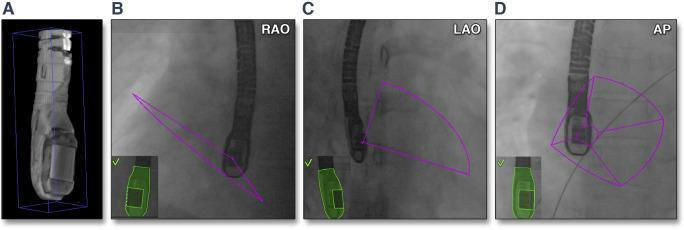
\includegraphics[width=6.30221in,height=2.25in]{immagini/image5.jpg}

\textbf{Figura 2. Co-registrazione eco-fluoroscopica: modello tridimensionale della sonda TEE (A), allineamento nelle proiezioni fluoroscopiche (B-C) e settore di acquisizione ecocardiografica (D). Riprodotta da Clegg et al. {[}22{]}, fig. 1. © 2015 American College of Cardiology Foundation, con autorizzazione tramite Elsevier.}\footnote{Reprinted from JACC: Cardiovascular Imaging, Vol. 8, Clegg SD, Chen SJ, Nijhof N, Kim MS, Salcedo EE, Quaife RA, Messenger JC, Bracken J, Carroll JD, ``Integrated 3D Echo-X Ray to Optimize Image Guidance for Structural Heart Intervention'', pp. 371--374, Copyright (2015), with permission from the American College of Cardiology Foundation.}

\hypertarget{riparazione-transcatetere-edge-to-edge-della-valvola-mitrale}{%
\subsection*{2.2 Riparazione transcatetere edge-to-edge della valvola mitrale}\label{riparazione-transcatetere-edge-to-edge-della-valvola-mitrale}}

Il fusion imaging può fornire un supporto in diverse fasi delle procedure transcatetere edge-to-edge delle valvole atrioventricolari, dall'individuazione dei reperi anatomici alla navigazione e al posizionamento del dispositivo. Le sue modalità di applicazione variano in base alla valvola trattata e al dispositivo impiegato. {[}1{]}

Poiché tutti gli studi inclusi nella presente revisione comprendevano pazienti sottoposti a riparazione transcatetere edge-to-edge della valvola mitrale mediante MitraClip, si è scelto di approfondire le principali fasi di questa procedura.

Nei sottoparagrafi successivi vengono pertanto descritte le viste ecocardiografiche e le proiezioni fluoroscopiche utilizzate durante la guida convenzionale. Queste costituiscono la base anche per l'impiego del fusion imaging, che ne consente la co-registrazione e la visualizzazione integrata. {[}1, 23{]}

\hypertarget{puntura-transettale-e-marker}{%
\subsubsection*{\texorpdfstring{\textbf{2.2.1 Puntura transettale e marker} }{2.2.1 Puntura transettale e marker }}\label{puntura-transettale-e-marker}}

La puntura transettale rappresenta una fase fondamentale nelle procedure mitraliche eseguite mediante accesso transvenoso, poiché permette il passaggio dall'atrio destro all'atrio sinistro attraverso il setto interatriale. {[}16, 23{]}

Le principali viste ottenute mediante ecocardiografia transesofagea per guidare la puntura transettale sono la vista bicavale, la vista medio-esofagea in asse corto a livello della valvola aortica e la vista medio-esofagea a quattro camere. {[}16, 23{]}

La vista bi-cavale permette di valutare l'orientamento superiore-inferiore, mostrando contemporaneamente la vena cava inferiore, la vena cava superiore, i due atri e il setto interatriale.

La vista in asse corto a livello della base consente invece di stabilire la posizione anteriore o posteriore del punto di puntura, utilizzando la radice aortica come riferimento anteriore.

Infine, la vista quattro camere mostra entrambi gli atri e i ventricoli e permette di valutare l'altezza del punto di puntura rispetto al piano della valvola mitrale. Le diverse viste permettono inoltre di controllare la posizione e l'avanzamento delle guide e dei cateteri e di valutarne i rapporti con le strutture cardiache. {[}16{]}

È utile sovrapporre una ricostruzione 3D del setto interatriale all'immagine fluoroscopica in proiezione RAO, per ottenere una vista \emph{en face} della fossa ovale e individuare un punto per la puntura nella sua porzione postero-superiore. {[}2{]}

Durante questa fase possono essere utilizzate le proiezioni fluoroscopiche antero-posteriore (AP) e obliqua anteriore sinistra (LAO). In quest'ultima, il fusion imaging consente di sovrapporre la corrispondente vista TEE bicavale. {[}2, 23{]}

\hypertarget{navigazione-dei-cateteri-e-dei-sistemi-di-rilascio}{%
\subsubsection*{\texorpdfstring{\textbf{2.2.2 Navigazione dei cateteri e dei sistemi di rilascio}}{2.2.2 Navigazione dei cateteri e dei sistemi di rilascio}}\label{navigazione-dei-cateteri-e-dei-sistemi-di-rilascio}}

Durante l'introduzione e l'avanzamento del catetere guida orientabile nell'atrio sinistro, la fluoroscopia viene generalmente acquisita nelle proiezioni antero-posteriore (AP) e RAO craniale. {[}2, 23{]}

Contemporaneamente, la TEE utilizza le viste medio-esofagee in asse corto, in asse lungo e a quattro camere, insieme alle ricostruzioni tridimensionali dell'atrio sinistro per valutare i rapporti spaziali del catetere con il setto interatriale, la parete atriale e il piano della valvola mitrale. {[}23{]}

Sulle immagini ecocardiografiche possono essere posizionati tre marker anatomici che, una volta trasferiti sull'immagine fluoroscopica, delimitano un triangolo virtuale utile alla navigazione del sistema. I marker identificano il sito ideale della puntura transettale, la cresta dell'atrio sinistro (\emph{left atrial ridge}), che separa l'auricola sinistra dalla vena polmonare superiore sinistra, e il centro della valvola mitrale. In questo modo, durante la navigazione nell'atrio sinistro, l'operatore dispone di riferimenti anatomici direttamente visibili sull'immagine fluoroscopica. {[}21{]}

\hypertarget{allineamento-e-posizionamento-del-dispositivo}{%
\subsubsection*{\texorpdfstring{\textbf{2.2.3 Allineamento e posizionamento del dispositivo}}{2.2.3 Allineamento e posizionamento del dispositivo}}\label{allineamento-e-posizionamento-del-dispositivo}}

Durante la navigazione verso la valvola mitrale, il sistema di rilascio viene posizionato al di sopra della sede del rigurgito. Le immagini fluoroscopiche vengono acquisite in proiezione obliqua anteriore destra (RAO) con angolazione craniale, mentre la TEE utilizza

la ricostruzione tridimensionale dell'atrio sinistro per seguire gli spostamenti principali del sistema e l'acquisizione biplanare, definita ``vista di traiettoria 2D'' per effettuare regolazioni più precise. Quest'ultima associa la vista intercommissurale, nella quale si visualizzano distintamente tre segmenti, alla corrispondente vista ortogonale in asse lungo, permettendo di controllare rispettivamente gli spostamenti medio-laterali e antero-posteriori. {[}23{]}

Prima dell'avanzamento nel ventricolo sinistro, il sistema di rilascio deve essere allineato perpendicolarmente al piano della valvola mitrale. Successivamente, i bracci della clip vengono orientati perpendicolarmente alla linea di coaptazione mediante la vista tridimensionale \emph{en face} e l'acquisizione biplanare. Nel posizionamento centrale, il corretto orientamento è confermato quando i bracci non sono visibili nella vista intercommissurale e nella proiezione RAO craniale, mentre risultano evidenti nella loro completa estensione nella vista in asse lungo del tratto di efflusso del ventricolo sinistro (\emph{left ventricular outflow tract}, LVOT). {[}23{]}

\hypertarget{cattura-dei-lembi-rilascio-e-controllo-finale}{%
\subsubsection*{\texorpdfstring{\textbf{2.2.4 Cattura dei lembi, rilascio e controllo finale}}{2.2.4 Cattura dei lembi, rilascio e controllo finale}}\label{cattura-dei-lembi-rilascio-e-controllo-finale}}

Il \emph{grasping} viene controllato in tempo reale mediante acquisizione TEE biplanare e fluoroscopia in proiezione RAO craniale. {[}23{]}

Dopo la cattura dei lembi, vengono verificati l'adeguato inserimento dei lembi e la stabilità del dispositivo mediante diverse viste bidimensionali e ricostruzioni tridimensionali. {[}23{]}

Prima del rilascio definitivo, il risultato viene valutato attraverso la stima del rigurgito residuo mediante color Doppler e la misurazione del gradiente transmitralico mediante Doppler continuo per identificare un'eventuale stenosi mitralica iatrogena. {[}23{]}

Dopo il rilascio vengono nuovamente valutati la stabilità del dispositivo e il risultato complessivo della riparazione. {[}23{]}

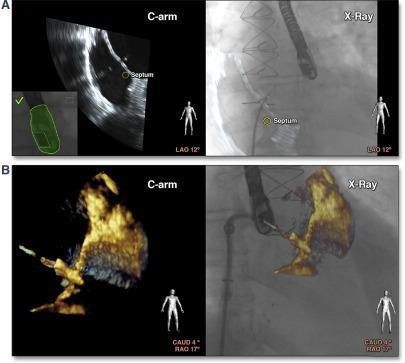
\includegraphics[width=4.59281in,height=3.58304in]{immagini/image4.jpg}

\textbf{Figura 3. Sovrapposizione delle immagini ecocardiografiche e fluoroscopiche durante il cateterismo transettale (A) e il posizionamento della MitraClip (B). Riprodotta da Clegg et al. {[}22{]}, fig. 3. © 2015 American College of Cardiology Foundation, con autorizzazione tramite Elsevier.}\footnote{Reprinted from JACC: Cardiovascular Imaging, Vol. 8, Clegg SD, Chen SJ, Nijhof N, Kim MS, Salcedo EE, Quaife RA, Messenger JC, Bracken J, Carroll JD, ``Integrated 3D Echo-X Ray to Optimize Image Guidance for Structural Heart Intervention'', pp. 371--374, Copyright (2015), with permission from the American College of Cardiology Foundation.}

\hypertarget{ruolo-del-tsrm}{%
\subsection*{2.3 Ruolo del TSRM}\label{ruolo-del-tsrm}}

La conoscenza dell'anatomia nelle immagini fluoroscopiche ed ecocardiografiche favorisce una comunicazione efficace tra i componenti del team di emodinamica. {[}2{]}

Sulla base di questi aspetti, si può ipotizzare che il TSRM, nell'ambito delle proprie competenze e in collaborazione con l'équipe, possa contribuire alla verifica del corretto allineamento tra le immagini ecocardiografiche e fluoroscopiche durante l\textquotesingle intervento. A questo scopo può controllare il colore del contorno della sonda sul monitor e prestare attenzione ai movimenti verticali del tavolo e agli spostamenti del paziente, che potrebbero rendere necessarie la verifica o la ripetizione della co-registrazione. Può inoltre collaborare con l'ecografista nel controllo della corrispondenza dei marker tra le due immagini prima che vengano confermati.

Una formazione specifica in anatomia ecocardiografica potrebbe valorizzare il contributo del tecnico di radiologia durante la procedura, facilitando la comprensione delle strutture cardiache e del loro orientamento spaziale al variare delle proiezioni fluoroscopiche e delle viste ecocardiografiche. Tale preparazione potrebbe risultare particolarmente utile durante la puntura transettale, consentendo al tecnico di comprendere, per esempio, la corrispondenza tra il \emph{tenting} del setto interatriale identificato dall'ecografista e la sua rappresentazione sovrapposta all'immagine fluoroscopica.

\clearpage
\hypertarget{materiali-e-metodi-della-revisione-sistematica}{%
\section*{3. Materiali e metodi della revisione sistematica}\label{materiali-e-metodi-della-revisione-sistematica}}

La visualizzazione integrata delle due metodiche su un unico monitor può facilitare l'individuazione dei punti anatomici di interesse, la navigazione e l'orientamento dei dispositivi e il controllo delle principali fasi procedurali. Inoltre, semplificando alcune fasi dell'intervento, il fusion imaging potrebbe contribuire alla riduzione dei tempi di fluoroscopia e dell'esposizione alle radiazioni ionizzanti del paziente e degli operatori. {[}1, 2{]}

Pertanto, nei pazienti adulti sottoposti a procedure transcatetere sulle valvole atrioventricolari, l'impiego del fusion imaging ecocardiografico-fluoroscopico, rispetto alla guida convenzionale basata sulla visualizzazione separata, è associato a una riduzione dell'esposizione alle radiazioni ionizzanti e dei tempi procedurali, nonché a un miglioramento del successo procedurale e della sicurezza?

La presente revisione sistematica è stata condotta secondo le raccomandazioni PRISMA 2020 (Preferred Reporting Items for Systematic Reviews and Meta-Analyses), al fine di garantire trasparenza e completezza nella descrizione del processo metodologico e di favorire la riproducibilità. {[}29{]}

Per definire in modo strutturato la domanda di ricerca è stato utilizzato il modello PICO. \hl{}

{\fontsize{10}{12}\selectfont\setlength{\tabcolsep}{3pt}
\begin{longtable}[]{@{}
  >{\raggedright\arraybackslash}p{(\columnwidth - 2\tabcolsep) * \real{0.1882}}
  >{\raggedright\arraybackslash}p{(\columnwidth - 2\tabcolsep) * \real{0.8118}}@{}}
\toprule\noalign{}
\begin{minipage}[b]{\linewidth}\raggedright
\textbf{Popolazione}
\end{minipage} & \begin{minipage}[b]{\linewidth}\raggedright
Pazienti adulti sottoposti a procedure valvolari transcatetere per patologia della valvola mitrale o tricuspide.
\end{minipage} \\
\begin{minipage}[b]{\linewidth}\raggedright
\textbf{Intervento}
\end{minipage} & \begin{minipage}[b]{\linewidth}\raggedright
Guida mediante fusion imaging ecocardiografico-fluoroscopico.
\end{minipage} \\
\begin{minipage}[b]{\linewidth}\raggedright
\textbf{Confronto}
\end{minipage} & \begin{minipage}[b]{\linewidth}\raggedright
Procedura guidata con fluoroscopia ed ecocardiografia transesofagea convenzionali senza software di fusion imaging.
\end{minipage} \\
\begin{minipage}[b]{\linewidth}\raggedright
\textbf{Outcome}
\end{minipage} & \begin{minipage}[b]{\linewidth}\raggedright
Tempo procedurale, tempo di fluoroscopia, esposizione alle radiazioni ionizzanti, successo procedurale, complicanze, sicurezza e indicatori di efficienza del workflow.
\end{minipage} \\
\midrule\noalign{}
\endhead
\bottomrule\noalign{}
\endlastfoot
\end{longtable}
}

\textbf{Tabella 1. Formulazione del quesito di ricerca secondo il modello PICO (Population, Intervention, Comparison e Outcome).}

\hypertarget{ricerca-bibliografica}{%
\subsection*{3.1 Ricerca bibliografica}\label{ricerca-bibliografica}}

Prima dell'avvio della ricerca bibliografica è stata effettuata una ricerca preliminare nel registro PROSPERO (International Prospective Register of Systematic Reviews), con l'obiettivo di accertare l'eventuale presenza di revisioni sistematiche già registrate, in corso di svolgimento o pubblicate sul medesimo quesito di ricerca. A tale scopo, sono state interrogate le registrazioni mediante le stringhe ``Fusion imaging'' AND (``mitral valve'' OR ``tricuspid valve'') ed ``EchoNavigator'', che non hanno restituito alcuna registrazione pertinente. La ricerca condotta utilizzando il solo termine ``fusion imaging'' ha identificato complessivamente 17 registrazioni. La valutazione dei relativi titoli e contenuti ha tuttavia evidenziato l'assenza di revisioni sistematiche caratterizzate da un quesito di ricerca sovrapponibile a quello oggetto della presente revisione, in termini di popolazione, intervento, comparatore e outcome considerati.

\hypertarget{metodo-di-conduzione-della-revisione-sistematica}{%
\subsection*{3.2 Metodo di conduzione della revisione sistematica}\label{metodo-di-conduzione-della-revisione-sistematica}}

Inizialmente sono state selezionate le banche dati contenenti studi scientifici di ambito medico, tenendo conto anche delle risorse accessibili tramite il profilo universitario: Web of Science, PubMed, Scopus e Health \& Medical Collection.

Per ognuna delle banche dati è stata inserita la medesima stringa: ("Fusion Imaging" OR "Echocardiographic Fluoroscopic Fusion" OR "Echocardiography-Fluoroscopy Fusion" OR "Echocardiographic-Fluoroscopic Fusion" OR "Echo-Fluoro Fusion" OR "Echo Fluoro Fusion" OR EchoNavigator OR "Echo Navigator") AND ("Mitral Valve" OR "Tricuspid Valve" OR "Transcatheter Mitral" OR "Percutaneous Mitral" OR "Transcatheter Tricuspid" OR "Percutaneous Tricuspid" OR "Transcatheter Edge-to-Edge Repair" OR "Transcatheter Edge to Edge Repair" OR TEER OR T-TEER OR TMVR OR TTVR OR MitraClip OR TriClip OR PASCAL OR EVOQUE OR Intrepid).

Al fine di procedere a una prima selezione dei risultati ottenuti, sono stati applicati specifici filtri bibliografici, differenziati in relazione alle caratteristiche delle singole banche dati.

{\fontsize{10}{12}\selectfont\setlength{\tabcolsep}{3pt}
\begin{longtable}[]{@{}
  >{\raggedright\arraybackslash}p{(\columnwidth - 2\tabcolsep) * \real{0.3250}}
  >{\raggedright\arraybackslash}p{(\columnwidth - 2\tabcolsep) * \real{0.6750}}@{}}
\toprule\noalign{}
\begin{minipage}[b]{\linewidth}\raggedright
\textbf{Banca dati}
\end{minipage} & \begin{minipage}[b]{\linewidth}\raggedright
\textbf{Filtri applicati}
\end{minipage} \\
\begin{minipage}[b]{\linewidth}\raggedright
Web of Science
\end{minipage} & \begin{minipage}[b]{\linewidth}\raggedright
Anni 2016-2026; esclusione dei \emph{Review Article}.
\end{minipage} \\
\begin{minipage}[b]{\linewidth}\raggedright
PubMed
\end{minipage} & \begin{minipage}[b]{\linewidth}\raggedright
Anni 2016-2026; disponibilità del \emph{full text}.
\end{minipage} \\
\begin{minipage}[b]{\linewidth}\raggedright
Scopus
\end{minipage} & \begin{minipage}[b]{\linewidth}\raggedright
Anni 2016-2026; articoli in lingua inglese; esclusione di \emph{review}, editoriali, capitoli di libro e \emph{short survey}.
\end{minipage} \\
\begin{minipage}[b]{\linewidth}\raggedright
Health \& Medical Collection
\end{minipage} & \begin{minipage}[b]{\linewidth}\raggedright
Anni 2016-2026; disponibilità del testo completo.
\end{minipage} \\
\midrule\noalign{}
\endhead
\bottomrule\noalign{}
\endlastfoot
\end{longtable}
}

\textbf{Tabella 2. Applicazione dei filtri al momento della ricerca bibliografica.}

\hypertarget{criteri-di-eleggibilituxe0-inclusione-ed-esclusione}{%
\subsubsection*{\texorpdfstring{\textbf{3.2.1 Criteri di eleggibilità, inclusione ed esclusione} }{3.2.1 Criteri di eleggibilità, inclusione ed esclusione }}\label{criteri-di-eleggibilituxe0-inclusione-ed-esclusione}}

Per la selezione degli studi sono stati stabiliti specifici criteri di eleggibilità, definiti in coerenza con la domanda di ricerca e con il modello PICO.

Per quanto concerne il disegno e la tipologia degli studi, sono stati considerati eleggibili esclusivamente gli studi clinici originali caratterizzati dalla presenza di un gruppo di confronto sottoposto alla medesima procedura mediante guida convenzionale, ossia in assenza di impiego del \emph{fusion imaging}.

La popolazione di interesse era costituita da pazienti adulti sottoposti a procedure transcatetere per il trattamento di patologie della valvola mitrale e/o tricuspide. Sono stati pertanto inclusi gli studi riguardanti procedure di riparazione transcatetere edge-to-edge (TEER) e di riparazione o sostituzione transcatetere delle valvole mitrale o tricuspide, indipendentemente dal dispositivo impiegato, purché riconducibile a sistemi quali MitraClip, TriClip, PASCAL, EVOQUE o Intrepid. Gli studi relativi alla chiusura percutanea dell'auricola sinistra (LAAO) o al trattamento dei leak paravalvolari sono stati considerati eleggibili solo se comprendevano popolazioni miste con pazienti sottoposti anche a procedure transcatetere mitraliche o tricuspidali.

Per quanto riguarda l'intervento di interesse, sono stati inclusi gli studi che valutavano l'impiego del fusion imaging ecocardiografico-fluoroscopico come modalità di guida intraprocedurale, in confronto alla guida convenzionale.

Sono stati definiti specifici criteri di esclusione, applicati in relazione alla tipologia di pubblicazione, alla popolazione o al modello studiato, alla procedura oggetto di valutazione e alla modalità di imaging impiegata.

Per quanto concerne la tipologia di pubblicazione, sono state escluse tutte le pubblicazioni non rispondenti ai criteri di eleggibilità, tra cui revisioni narrative o sistematiche, meta-analisi, \emph{state-of-the-art review}, editoriali e commenti, linee guida e documenti di consenso, protocolli di studio, \emph{case report} e \emph{case series}, abstract congressuali e \emph{conference proceedings}, capitoli di libro, immagini cliniche, \emph{video article}, lettere e note prive di dati clinici comparativi originali, nonché tesi e dissertazioni.

Relativamente alla popolazione e al modello di studio, sono stati esclusi gli studi condotti su popolazioni pediatriche, modelli animali e preclinici, nonché studi in vitro, ex vivo, su cadavere o phantom. Sono stati inoltre esclusi studi basati esclusivamente su simulazioni, modelli computazionali o valutazioni di carattere esclusivamente tecnico, in assenza di pazienti sottoposti alla procedura oggetto di studio.

Per quanto riguarda la tipologia di procedura, non sono stati considerati eleggibili gli studi relativi a procedure transcatetere della valvola aortica, incluse TAVI/TAVR, né quelli riguardanti la valvola polmonare, gli interventi coronarici o elettrofisiologici, le procedure per il trattamento delle cardiopatie congenite, la chiusura dei difetti settali e le procedure di cardiochirurgia. Sono stati altresì esclusi gli studi focalizzati esclusivamente sulla chiusura percutanea dell'auricola sinistra (LAAO/LAAC) o sul trattamento dei leak paravalvolari.

Infine, in relazione alla modalità di imaging, sono stati esclusi gli studi nei quali non fosse impiegato il fusion imaging ecocardiografico-fluoroscopico. Non sono state pertanto considerate pertinenti le pubblicazioni riguardanti tecniche di fusione tra modalità di imaging differenti, quali CT-fluoroscopia, CBCT-fluoroscopia o MRI-fluoroscopia, né quelle basate esclusivamente sull'impiego di roadmap tridimensionali, in assenza di un'integrazione dinamica e in tempo reale tra immagini ecocardiografiche e fluoroscopiche.

{\fontsize{10}{12}\selectfont\setlength{\tabcolsep}{3pt}
\begin{longtable}[]{@{}
  >{\raggedright\arraybackslash}p{(\columnwidth - 4\tabcolsep) * \real{0.2126}}
  >{\raggedright\arraybackslash}p{(\columnwidth - 4\tabcolsep) * \real{0.3953}}
  >{\raggedright\arraybackslash}p{(\columnwidth - 4\tabcolsep) * \real{0.3920}}@{}}
\toprule\noalign{}
\begin{minipage}[b]{\linewidth}\raggedright
\end{minipage} & \begin{minipage}[b]{\linewidth}\raggedright
\textbf{Criteri di inclusione}
\end{minipage} & \begin{minipage}[b]{\linewidth}\raggedright
\textbf{Criteri di esclusione}
\end{minipage} \\
\begin{minipage}[b]{\linewidth}\raggedright
\textbf{Tipo di pubblicazione e disegno dello studio.}
\end{minipage} & \begin{minipage}[b]{\linewidth}\raggedright
Studi clinici originali.
\end{minipage} & \begin{minipage}[b]{\linewidth}\raggedright
Revisioni narrative o sistematiche; meta-analisi; \emph{state-of-the-art review}; editoriali e commenti; linee guida e documenti di consenso; protocolli di studio\emph{; case report} e \emph{case series}; abstract congressuali e \emph{conference proceedings}; capitoli di libro; immagini cliniche; \emph{video article}; lettere e note prive di dati clinici comparativi originali; tesi e dissertazioni.
\end{minipage} \\
\begin{minipage}[b]{\linewidth}\raggedright
\textbf{Popolazione}
\end{minipage} & \begin{minipage}[b]{\linewidth}\raggedright
Pazienti adulti.
\end{minipage} & \begin{minipage}[b]{\linewidth}\raggedright
Pazienti pediatrici, modelli animali e preclinici, nonché studi in vitro, ex vivo, su cadavere o phantom, su simulazioni, modelli computazionali o esclusivamente tecnici.
\end{minipage} \\
\begin{minipage}[b]{\linewidth}\raggedright
\textbf{Procedure}
\end{minipage} & \begin{minipage}[b]{\linewidth}\raggedright
Riparazione transcatetere edge-to-edge (TEER) e riparazione o sostituzione transcatetere delle valvole mitrale o tricuspide con dispositivi quali MitraClip, TriClip, PASCAL, EVOQUE o Intrepid. La chiusura percutanea dell\textquotesingle auricola sinistra (LAAO/LAAC) e il trattamento dei leak paravalvolari sono eleggibili solo qualora la popolazione fosse mista e includesse anche le procedure transcatetere delle valvole atrioventricolari.
\end{minipage} & \begin{minipage}[b]{\linewidth}\raggedright
Procedure transcatetere della valvola aortica (TAVI/TAVR), della valvola polmonare. Interventi coronarici o elettrofisiologici, per il trattamento di cardiopatie congenite e cardiochirurgici. Studi esclusivamente incentrati sulla chiusura percutanea dell\textquotesingle auricola sinistra (LAAO/LAAC) o sul trattamento dei leak paravalvolari.
\end{minipage} \\
\begin{minipage}[b]{\linewidth}\raggedright
\textbf{Intervento}
\end{minipage} & \begin{minipage}[b]{\linewidth}\raggedright
Fusion imaging real-time ecocardiografico-fluoroscopico.
\end{minipage} & \begin{minipage}[b]{\linewidth}\raggedright
Fusion imaging CT-fluoroscopia, CBCT-fluoroscopia o MRI-fluoroscopia. Impiego esclusivo di roadmap tridimensionali senza l\textquotesingle integrazione dinamica e in tempo reale tra le immagini ecocardiografiche-fluoroscopiche.
\end{minipage} \\
\midrule\noalign{}
\endhead
\bottomrule\noalign{}
\endlastfoot
\end{longtable}
}

\textbf{Tabella 3. Criteri di inclusione e di esclusione adottati per la selezione degli studi.}

\hypertarget{estrazione-dati}{%
\subsubsection*{\texorpdfstring{\textbf{3.2.2 Estrazione dati}}{3.2.2 Estrazione dati}}\label{estrazione-dati}}

Durante la lettura dei testi completi, i dati di interesse sono stati raccolti mediante Fogli Google. Per ciascuno studio sono stati estratti gli autori, il Paese, il disegno dello studio e le informazioni relative agli elementi del PICO, tra cui la procedura adottata, la numerosità e le caratteristiche del campione, l'intervento e il gruppo di controllo. Sono stati inoltre raccolti i principali outcome: il tempo procedurale, il tempo di fluoroscopia, l'esposizione alle radiazioni ionizzanti, il successo procedurale e le complicanze.

\clearpage
\hypertarget{risultati}{%
\section*{4. Risultati}\label{risultati}}

\hypertarget{selezione-degli-articoli}{%
\subsection*{\texorpdfstring{4.1 Selezione degli articoli }{4.1 Selezione degli articoli }}\label{selezione-degli-articoli}}

A seguito dell'applicazione dei filtri, sono stati complessivamente identificati 68 risultati in Web of Science, 52 in PubMed, 49 in Scopus e 266 nella banca dati Health \& Medical Collection (ProQuest).

I 435 record individuati attraverso la ricerca nelle banche dati selezionate sono stati inizialmente esportati su Zotero e successivamente caricati sulla piattaforma Rayyan. Il software ha individuato 156 record come potenziali duplicati sulla base della corrispondenza di elementi quali il DOI, il titolo e gli autori.

Tutti i record segnalati sono stati verificati manualmente: 15 non sono stati considerati duplicati, mentre 62 record sono stati mantenuti poiché rappresentavano la versione più completa rispetto al corrispondente duplicato. Complessivamente, sono stati rimossi 79 record duplicati.

Al termine di questa procedura sono rimasti 356 record, sottoposti allo screening del titolo e dell'abstract.

Applicando in ordine gerarchico i criteri di esclusione prestabiliti e attribuendo a ciascun record un unico motivo principale di esclusione, ne sono stati esclusi 352.

In particolare, 283 articoli sono stati esclusi per tipo di pubblicazione non eleggibile, 9 per popolazione o modello non eleggibile, 34 perché la valvola in studio o la procedura non erano pertinenti e 26 perché l'intervento di imaging non corrispondeva a quello previsto dalla domanda di ricerca.

Al termine di questa fase, quattro articoli sono stati considerati potenzialmente eleggibili e sottoposti alla valutazione del testo completo.

In seguito alla lettura del testo completo dei quattro articoli rimasti, uno è stato escluso perché presentava un disegno non comparativo e non prevedeva, quindi, un gruppo di controllo sottoposto a guida convenzionale con cui confrontare gli outcome associati all'impiego del fusion imaging.

Al termine del processo di selezione sono stati inclusi tre studi, successivamente sottoposti all'estrazione e all'analisi dei dati. {[}24, 25, 26{]}

{\fontsize{10}{12}\selectfont\setlength{\tabcolsep}{3pt}
\begin{longtable}[]{@{}
  >{\raggedright\arraybackslash}p{(\columnwidth - 4\tabcolsep) * \real{0.2027}}
  >{\raggedright\arraybackslash}p{(\columnwidth - 4\tabcolsep) * \real{0.3467}}
  >{\raggedright\arraybackslash}p{(\columnwidth - 4\tabcolsep) * \real{0.4506}}@{}}
\toprule\noalign{}
\begin{minipage}[b]{\linewidth}\raggedright
\textbf{Record totali ricerca}
\end{minipage} & \begin{minipage}[b]{\linewidth}\raggedright
\textbf{Duplicati rimossi}
\end{minipage} & \begin{minipage}[b]{\linewidth}\raggedright
\textbf{Record rimasti dopo eliminazione duplicati}
\end{minipage} \\
\begin{minipage}[b]{\linewidth}\raggedright
435
\end{minipage} & \begin{minipage}[b]{\linewidth}\raggedright
79
\end{minipage} & \begin{minipage}[b]{\linewidth}\raggedright
356
\end{minipage} \\
\midrule\noalign{}
\endhead
\bottomrule\noalign{}
\endlastfoot
\end{longtable}
}

\textbf{Tabella 4. Numero di record identificati e rimasti dopo l'eliminazione dei duplicati.}

{\fontsize{10}{12}\selectfont\setlength{\tabcolsep}{3pt}
\begin{longtable}[]{@{}
  >{\raggedright\arraybackslash}p{(\columnwidth - 4\tabcolsep) * \real{0.2140}}
  >{\raggedright\arraybackslash}p{(\columnwidth - 4\tabcolsep) * \real{0.3729}}
  >{\raggedright\arraybackslash}p{(\columnwidth - 4\tabcolsep) * \real{0.4130}}@{}}
\toprule\noalign{}
\begin{minipage}[b]{\linewidth}\raggedright
\end{minipage} & \begin{minipage}[b]{\linewidth}\raggedright
\textbf{Record esclusi mediante screening titolo/abstract}
\end{minipage} & \begin{minipage}[b]{\linewidth}\raggedright
\textbf{Record esclusi mediante screening lettura full text}
\end{minipage} \\
\begin{minipage}[b]{\linewidth}\raggedright
\textbf{Tipo di pubblicazione o disegno di studio non eleggibile}
\end{minipage} & \begin{minipage}[b]{\linewidth}\raggedright
283
\end{minipage} & \begin{minipage}[b]{\linewidth}\raggedright
1
\end{minipage} \\
\begin{minipage}[b]{\linewidth}\raggedright
\textbf{Popolazione o modello non eleggibile}
\end{minipage} & \begin{minipage}[b]{\linewidth}\raggedright
9
\end{minipage} & \begin{minipage}[b]{\linewidth}\raggedright
\end{minipage} \\
\begin{minipage}[b]{\linewidth}\raggedright
\textbf{Valvola in studio o procedura non pertinenti}
\end{minipage} & \begin{minipage}[b]{\linewidth}\raggedright
34
\end{minipage} & \begin{minipage}[b]{\linewidth}\raggedright
\end{minipage} \\
\begin{minipage}[b]{\linewidth}\raggedright
\textbf{Intervento non pertinente}
\end{minipage} & \begin{minipage}[b]{\linewidth}\raggedright
26
\end{minipage} & \begin{minipage}[b]{\linewidth}\raggedright
\end{minipage} \\
\begin{minipage}[b]{\linewidth}\raggedright
\textbf{Totale}
\end{minipage} & \begin{minipage}[b]{\linewidth}\raggedright
352
\end{minipage} & \begin{minipage}[b]{\linewidth}\raggedright
1
\end{minipage} \\
\midrule\noalign{}
\endhead
\bottomrule\noalign{}
\endlastfoot
\end{longtable}
}

\textbf{Tabella 5. Distribuzione dei record esclusi durante lo screening del titolo e dell'abstract e durante la lettura del testo completo, suddivisi in base alla motivazione dell'esclusione.}

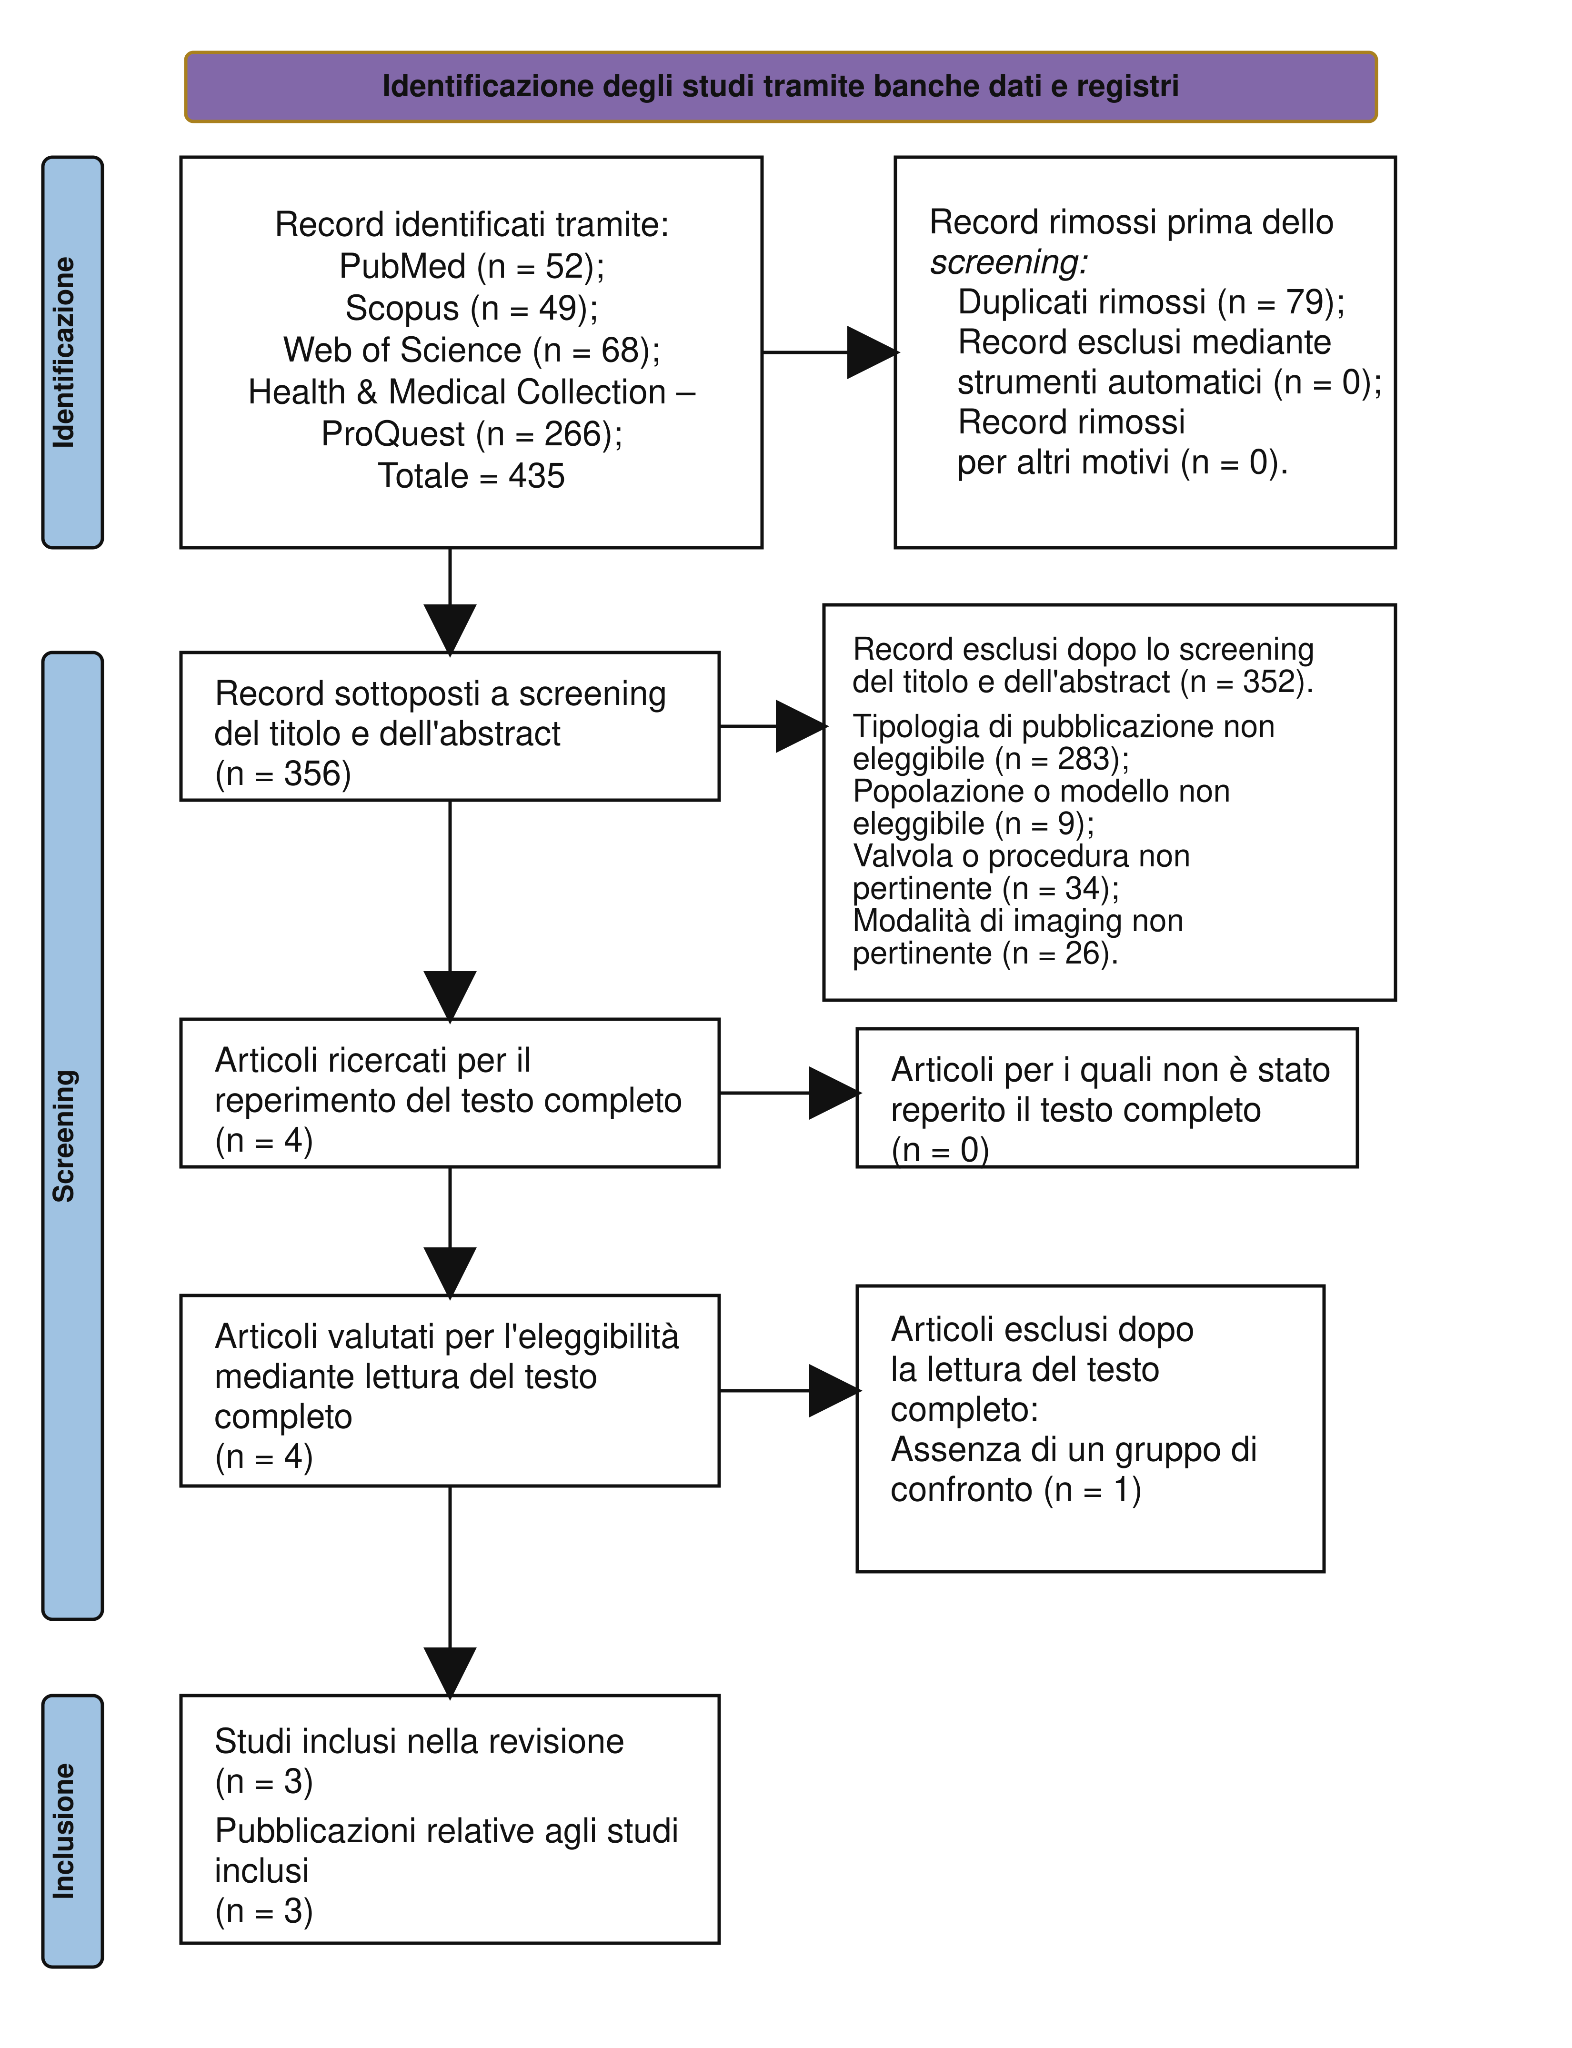
\includegraphics[width=\linewidth,height=.83\textheight,keepaspectratio]{immagini/image2.png}

\textbf{Figura 4. Diagramma di flusso PRISMA 2020 relativo al processo di selezione degli studi. Tradotto e adattato da Page et al. (2021), licenza CC BY 4.0. {[}29{]}}

\hypertarget{studi-inclusi}{%
\subsection*{4.2 Studi inclusi}\label{studi-inclusi}}

Tutti gli studi presentavano un disegno osservazionale, retrospettivo, monocentrico e comparativo di tipo before-after, con una coorte storica di controllo. {[}24, 25, 26{]}

Lo studio comparativo di Afzal et al. (2017) ha incluso retrospettivamente 88 pazienti adulti, sottoposti a procedure di interventistica cardiaca strutturale per impianto di MitraClip o per la chiusura dell'auricola sinistra (LAAO), e li ha suddivisi in due gruppi da 44 pazienti ciascuno. Un gruppo, denominato -EchoNav, è stato trattato mediante la tecnica di imaging tradizionale, nella quale le immagini fluoroscopiche ed ecocardiografiche venivano visualizzate separatamente. Il secondo gruppo, denominato +EchoNav, è stato trattato mediante fusion imaging in seguito all'introduzione nella pratica clinica del sistema EchoNavigator Release II (EchoNav II, Philips Healthcare, Andover, Massachusetts, USA). {[}24{]}

Ciascun gruppo comprendeva 16 procedure di impianto di MitraClip e 28 procedure di chiusura dell'auricola sinistra; i risultati relativi alle due tipologie di intervento sono pertanto riportati in forma aggregata. {[}24{]}

È stata osservata una riduzione statisticamente significativa del tempo compreso tra l'accesso vascolare femorale e l'esecuzione con successo della puntura transettale (FI+ = 18,48 ± 5,62 min; FI− = 23,20 ± 9,61 min; p = 0,006). {[}24{]}

La fattibilità tecnica del sistema di fusion imaging durante l'operazione di puntura transettale è stata valutata considerando il successo di tutte le TSP in entrambi i gruppi. {[}24{]}

La sicurezza è sostenuta dall'assenza di complicanze correlate alla puntura transettale. I due eventi avversi osservati si sono verificati successivamente e sono risultati indipendenti da essa. Entrambi si sono verificati durante la procedura di chiusura dell'auricola sinistra (LAAO): dislocazione occluder (FI+) e blocco atrioventricolare (BAV) III grado intermittente (FI−). {[}24{]}

Lo studio di Afzal et al. (2020) è un'analisi retrospettiva condotta su 194 pazienti consecutivi sottoposti a riparazione transcatetere edge-to-edge della valvola mitrale (M-TEER), successivamente suddivisi in due gruppi di studio.\\
Le procedure del primo gruppo (FI-), comprendente 99 pazienti, sono state eseguite con tecnica di imaging tradizionale, nella quale le immagini ecocardiografiche e fluoroscopiche venivano visualizzate separatamente. Il secondo gruppo, composto da 95 pazienti (FI+), è stato invece sottoposto alla procedura dopo l'installazione del sistema di fusion imaging EchoNavigator (Philips Healthcare, Best, the Netherlands). {[}25{]}

Il tempo necessario per completare con successo la puntura transettale con l'impiego del fusion imaging è risultato significativamente inferiore (FI+ = 26,1 ± 12,0 min; FI− = 35,2 ± 16,9 min; p \textless{} 0,001). {[}25{]}

Il tempo procedurale totale è risultato lievemente inferiore nel gruppo FI+, ma la differenza non è risultata statisticamente significativa (FI+ = 92,5 ± 32,3 min; FI− = 95,6 ± 36,2 min; p = 0,524). {[}25{]}

Anche la riduzione del tempo di fluoroscopia osservata nel gruppo FI+ non ha raggiunto la significatività statistica. {[}25{]}

Il kerma-area product (KAP), indicato nello studio come dose-area product (DAP), è risultato numericamente più elevato nel gruppo FI+, senza tuttavia evidenziare una differenza statisticamente significativa rispetto al gruppo FI-. {[}25{]}

Non sono state rilevate differenze statisticamente significative nell'incidenza delle complicanze, né nella mortalità a 30 giorni tra i due gruppi. {[}25{]}

Infine, l'analisi condotta sui pazienti che hanno richiesto l'impianto di più dispositivi non ha evidenziato differenze significative nei tempi procedurali tra i due gruppi. {[}25{]}

Lo studio di Melillo et al. (2021) ha incluso 160 pazienti affetti da insufficienza mitralica di grado da moderato a severo. Di questi ne furono analizzati 158 e di conseguenza 79 per gruppo. {[}26{]}

Per valutare la rilevanza del fusion imaging sul successo della riparazione transcatetere, sono stati costituiti due gruppi, FI- e FI+. I pazienti sono stati trattati dallo stesso team di cardiologi interventisti ed ecografisti esperti, rispettivamente prima e dopo l'installazione del sistema EchoNavigator versione 2 (Philips Medical System, Best, the Netherlands). {[}26{]}

Nella maggior parte dei casi è stata impiantata una sola clip, mentre nel 43,2\% dei pazienti è stato necessario impiantarne due; la distribuzione è risultata simile nei due gruppi. {[}26{]}

Dall'analisi del tempo necessario per completare la procedura è emersa una riduzione nel gruppo FI+, che tuttavia non ha raggiunto la significatività statistica. Al contrario, la riduzione del tempo di fluoroscopia osservata nel gruppo FI+ è risultata statisticamente significativa (FI+ = 37,3 ± 14,6 min; FI− = 48,3 ± 28,3 min; p = 0,003). {[}26{]}

Inoltre, il maggior successo procedurale riscontrato nel gruppo con fusion imaging è risultato statisticamente significativo sia al termine della procedura sia al momento della dimissione (fine procedura: FI+ = 91,1\% vs FI− = 79,7\%; p = 0,042; alla dimissione: FI+ = 77,2\% vs FI− = 61,5\%; p = 0,033). {[}26{]}

Il KAP registrato nei due gruppi non ha mostrato differenze statisticamente significative. Analogamente, non sono emerse differenze statisticamente significative nell'incidenza delle complicanze tra i due gruppi. {[}26{]}

{\fontsize{10}{12}\selectfont\setlength{\tabcolsep}{3pt}
\begin{longtable}[]{@{}
  >{\raggedright\arraybackslash}p{(\columnwidth - 10\tabcolsep) * \real{0.1120}}
  >{\raggedright\arraybackslash}p{(\columnwidth - 10\tabcolsep) * \real{0.1656}}
  >{\raggedright\arraybackslash}p{(\columnwidth - 10\tabcolsep) * \real{0.1957}}
  >{\raggedright\arraybackslash}p{(\columnwidth - 10\tabcolsep) * \real{0.1773}}
  >{\raggedright\arraybackslash}p{(\columnwidth - 10\tabcolsep) * \real{0.1672}}
  >{\raggedright\arraybackslash}p{(\columnwidth - 10\tabcolsep) * \real{0.1823}}@{}}
\toprule\noalign{}
\begin{minipage}[b]{\linewidth}\raggedright
\textbf{Studio}
\end{minipage} & \begin{minipage}[b]{\linewidth}\raggedright
\textbf{Disegno di studio}
\end{minipage} & \begin{minipage}[b]{\linewidth}\raggedright
\textbf{Procedura e campione}
\end{minipage} & \begin{minipage}[b]{\linewidth}\raggedright
\textbf{Intervento}
\end{minipage} & \begin{minipage}[b]{\linewidth}\raggedright
\textbf{Controllo}
\end{minipage} & \begin{minipage}[b]{\linewidth}\raggedright
\textbf{Outcome}
\end{minipage} \\
\begin{minipage}[b]{\linewidth}\raggedright
Afzal et al. (2017), Germania {[}24{]}
\end{minipage} & \begin{minipage}[b]{\linewidth}\raggedright
Studio osservazionale, retrospettivo, monocentrico e comparativo con disegno before-after e coorte storica di controllo.
\end{minipage} & \begin{minipage}[b]{\linewidth}\raggedright
Popolazione mista MitraClip/LAAO.

Totale di 88 pazienti:

FI- (before) = 44 e FI+ (after) = 44.

In ciascun gruppo: 16 procedure MitraClip e 28 LAAO.
\end{minipage} & \begin{minipage}[b]{\linewidth}\raggedright
Fusion imaging real-time con EchoNavigator system Release II (EchoNav II, Philips Healthcare, Andover, Massachusetts, USA).
\end{minipage} & \begin{minipage}[b]{\linewidth}\raggedright
Guida convenzionale con TEE e fluoroscopia visualizzate separatamente.
\end{minipage} & \begin{minipage}[b]{\linewidth}\raggedright
Eventi avversi correlati alla puntura transettale; successo della puntura nel sito prespecificato; tempo fino alla puntura transettale.
\end{minipage} \\
\begin{minipage}[b]{\linewidth}\raggedright
Afzal et al. (2020), Germania \hl{}{[}25{]}
\end{minipage} & \begin{minipage}[b]{\linewidth}\raggedright
Studio osservazionale, retrospettivo, monocentrico e comparativo con disegno before-after e coorte storica di controllo.
\end{minipage} & \begin{minipage}[b]{\linewidth}\raggedright
Riparazione mitralica transcatetere edge-to-edge con MitraClip.

Totale di 194 pazienti consecutivi: FI- (before) = 99 e FI+ (after) = 95.
\end{minipage} & \begin{minipage}[b]{\linewidth}\raggedright
Fusion imaging real-time con EchoNavigator (EchoNavigator System, Philips Healthcare, Best, the Netherlands).
\end{minipage} & \begin{minipage}[b]{\linewidth}\raggedright
Guida convenzionale con TEE e fluoroscopia visualizzate separatamente.
\end{minipage} & \begin{minipage}[b]{\linewidth}\raggedright
Tempo fino alla puntura transettale; tempo procedurale totale; tempo di fluoroscopia; dose-area product (DAP); eventi avversi.
\end{minipage} \\
\begin{minipage}[b]{\linewidth}\raggedright
Melillo et al. (2021), Italia {[}26{]}
\end{minipage} & \begin{minipage}[b]{\linewidth}\raggedright
Studio osservazionale, retrospettivo, monocentrico e comparativo con disegno before-after e coorte storica di controllo.
\end{minipage} & \begin{minipage}[b]{\linewidth}\raggedright
Riparazione mitralica transcatetere edge-to-edge con MitraClip.

Totale di 160 pazienti consecutivi inclusi ma 158 analizzati: FI- (before) = 79 e FI+ (after) = 79.
\end{minipage} & \begin{minipage}[b]{\linewidth}\raggedright
Fusion imaging real-time con EchoNavigator version 2 (Philips Medical System, Best, the Netherlands).
\end{minipage} & \begin{minipage}[b]{\linewidth}\raggedright
Guida convenzionale con TEE e fluoroscopia visualizzate separatamente.
\end{minipage} & \begin{minipage}[b]{\linewidth}\raggedright
Tempo di fluoroscopia; kerma-area product (KAP); tempo procedurale totale; successo procedurale; complicanze.
\end{minipage} \\
\midrule\noalign{}
\endhead
\bottomrule\noalign{}
\endlastfoot
\end{longtable}
}

\textbf{Tabella 6. Sintesi delle principali caratteristiche metodologiche e cliniche degli studi inclusi secondo il modello PICO. {[}24, 25, 26{]}}

{\fontsize{10}{12}\selectfont\setlength{\tabcolsep}{3pt}
\begin{longtable}[]{@{}
  >{\raggedright\arraybackslash}p{(\columnwidth - 10\tabcolsep) * \real{0.1080}}
  >{\raggedright\arraybackslash}p{(\columnwidth - 10\tabcolsep) * \real{0.2292}}
  >{\raggedright\arraybackslash}p{(\columnwidth - 10\tabcolsep) * \real{0.1561}}
  >{\raggedright\arraybackslash}p{(\columnwidth - 10\tabcolsep) * \real{0.1495}}
  >{\raggedright\arraybackslash}p{(\columnwidth - 10\tabcolsep) * \real{0.1578}}
  >{\raggedright\arraybackslash}p{(\columnwidth - 10\tabcolsep) * \real{0.1993}}@{}}
\toprule\noalign{}
\begin{minipage}[b]{\linewidth}\raggedright
\textbf{Studio}
\end{minipage} & \begin{minipage}[b]{\linewidth}\raggedright
\textbf{Tempo fino a TSP/procedurale}
\end{minipage} & \begin{minipage}[b]{\linewidth}\raggedright
\textbf{Fluoroscopia}
\end{minipage} & \begin{minipage}[b]{\linewidth}\raggedright
\textbf{DAP/KAP}
\end{minipage} & \begin{minipage}[b]{\linewidth}\raggedright
\textbf{Successo}
\end{minipage} & \begin{minipage}[b]{\linewidth}\raggedright
\textbf{Complicanze}
\end{minipage} \\
\begin{minipage}[b]{\linewidth}\raggedright
Afzal et al. (2017) {[}24{]}
\end{minipage} & \begin{minipage}[b]{\linewidth}\raggedright
Tempo fino a TSP:

FI+ = 18,48 ± 5,62 min;

FI− = 23,20 ± 9,61 min;

p = 0,006.

Tempo procedurale totale: NR.
\end{minipage} & \begin{minipage}[b]{\linewidth}\raggedright
NR
\end{minipage} & \begin{minipage}[b]{\linewidth}\raggedright
NR
\end{minipage} & \begin{minipage}[b]{\linewidth}\raggedright
Successo TSP nel sito prespecificato: FI+ = 44/44 (100\%);

FI− = 44/44 (100\%).
\end{minipage} & \begin{minipage}[b]{\linewidth}\raggedright
Nessun evento avverso correlato alla TSP.

Due eventi successivi e indipendenti dalla TSP.
\end{minipage} \\
\begin{minipage}[b]{\linewidth}\raggedright
Afzal et al. (2020) {[}25{]}
\end{minipage} & \begin{minipage}[b]{\linewidth}\raggedright
Tempo fino a TSP:

FI+ = 26,1 ± 12,0 min;

FI− = 35,2 ± 16,9 min;

p \textless{} 0,001.

Tempo procedurale totale:

FI+ = 92,5 ± 32,3 min;

FI− = 95,6 ± 36,2 min;

p = 0,524.
\end{minipage} & \begin{minipage}[b]{\linewidth}\raggedright
FI+ = 27,7 ± 13,1 min;

FI− = 30,1 ± 16,1 min;

p = 0,269.
\end{minipage} & \begin{minipage}[b]{\linewidth}\raggedright
DAP:

FI+ = 7.521,0 ± 5.221,26 cGy·cm²;

FI− = 6.351,6 ± 5.783,2 cGy·cm²;

p = 0,146.
\end{minipage} & \begin{minipage}[b]{\linewidth}\raggedright
NR
\end{minipage} & \begin{minipage}[b]{\linewidth}\raggedright
Mortalità a 30 giorni:

FI+ = 1\% vs

FI− = 2\%;

p = 0,585.

Sanguinamento maggiore sito accesso:

FI+ = 0\% vs

FI− = 1\%;

p = 0,326.

Danno renale acuto senza necessità di dialisi:

FI+ = 1,1\% vs

FI− = 1,0\%;

p = 0,977.
\end{minipage} \\
\begin{minipage}[b]{\linewidth}\raggedright
Melillo et al. (2021) {[}26{]}
\end{minipage} & \begin{minipage}[b]{\linewidth}\raggedright
Tempo TSP: NR.

Tempo procedurale totale:

FI+ = 92,2 ± 36,1 min;

FI− = 103,1 ± 42,7 min;

p = 0,086.
\end{minipage} & \begin{minipage}[b]{\linewidth}\raggedright
FI+ = 37,3 ± 14,6 min;

FI− = 48,3 ± 28,3 min;

p = 0,003.
\end{minipage} & \begin{minipage}[b]{\linewidth}\raggedright
KAP:

FI+ = 91,5 ± 74,1 Gy·cm²; FI− = 108,8 ± 105,0 Gy·cm²;

p = 0,23.
\end{minipage} & \begin{minipage}[b]{\linewidth}\raggedright
Fine procedura: FI+ = 91,1\% vs FI− = 79,7\%;

p = 0,042;

Alla dimissione: FI+ = 77,2\% vs FI− = 61,5\%;

p = 0,033.
\end{minipage} & \begin{minipage}[b]{\linewidth}\raggedright
Complicanze periprocedurali complessive:

FI+ = 8,9\% vs

FI− = 13,0\%

(p = 0,40).
\end{minipage} \\
\midrule\noalign{}
\endhead
\bottomrule\noalign{}
\endlastfoot
\end{longtable}
}

\textbf{Tabella 7. Sintesi comparativa degli outcome procedurali, dosimetrici e di sicurezza riportati negli studi inclusi. {[}24, 25, 26{]}}

Abbreviazioni: FI, fusion imaging; FI−, gruppo senza fusion imaging; FI+, gruppo con fusion imaging; LAAO, occlusione dell'auricola atriale sinistra; TEE, ecocardiografia transesofagea; DAP, dose-area product; KAP, kerma-area product; TSP, puntura transettale; NR, dato non riportato. Nota: Ai fini dell'interpretazione dei risultati riportati, valori di p \textless{} 0,05 sono stati considerati statisticamente significativi; valori di p ≥ 0,05 sono stati considerati non statisticamente significativi.

\hypertarget{valutazione-del-rischio-di-bias---robins-i-risk-of-bias-in-non-randomized-studies-of-interventions}{%
\subsection*{4.3 Valutazione del rischio di bias - ROBINS-I (Risk Of Bias In Non-randomized Studies of Interventions)}\label{valutazione-del-rischio-di-bias---robins-i-risk-of-bias-in-non-randomized-studies-of-interventions}}

Poiché tutti gli studi inclusi presentavano un disegno osservazionale non randomizzato, il rischio di bias è stato valutato mediante lo strumento ROBINS-I, versione 2016. {[}30{]}

Per ciascuno studio sono stati esaminati i sette domini relativi al confondimento, alla selezione dei partecipanti, alla classificazione degli interventi, alle deviazioni dagli interventi previsti, ai dati mancanti, alla misurazione degli outcome e alla selezione dei risultati riportati.

La criticità comune ai tre studi è il disegno comparativo before-after, che confronta pazienti trattati prima e dopo l'introduzione del fusion imaging. Tale disegno espone gli studi a un possibile confondimento temporale, dovuto all'esperienza progressivamente acquisita dall'équipe e agli eventuali cambiamenti nell'organizzazione della procedura. Le differenze osservate negli outcome non possono pertanto essere attribuite con certezza alla sola introduzione della tecnologia. Il possibile contributo della curva di apprendimento è stato affrontato con modalità differenti nei tre studi.

Lo studio di Afzal et al. (2017) non ha valutato direttamente l'effetto della curva di apprendimento. Gli autori hanno tuttavia ritenuto che gli operatori avessero già raggiunto una fase piatta della curva di apprendimento, sulla base dell'elevato numero di punture transettali eseguite prima dell'introduzione del fusion imaging. Tale considerazione non consente comunque di escludere un possibile confondimento temporale. {[}24{]}

Nello studio di Afzal et al. (2020) gli autori hanno invece eseguito un'analisi di covarianza per ogni parametro procedurale, al fine di valutare il possibile effetto della curva di apprendimento, considerando la data della procedura come covariata. Anche dopo l'aggiustamento statistico, la riduzione del tempo necessario per eseguire con successo la puntura transettale nel gruppo FI+ è rimasta statisticamente significativa. {[}25{]}

L'analisi di regressione lineare e il test non parametrico di Mann-Kendall per trend monotoni, condotti dagli autori dello studio di Melillo et al. (2021) per valutare la presenza di una possibile learning curve, non hanno evidenziato una riduzione statisticamente significativa del tempo procedurale e del kerma-area product con il susseguirsi delle procedure. Queste analisi non hanno rilevato un andamento temporale statisticamente significativo dei parametri considerati, ma non consentono di escludere completamente l'influenza dell'esperienza degli operatori. {[}26{]}

I co-interventi meritano altrettanta attenzione, considerando il loro possibile impatto sui risultati.

Nello studio di Melillo et al. (2021) era presente uno sbilanciamento tra i due gruppi relativo al tipo di dispositivo MitraClip impiegato: tutti i pazienti del gruppo FI- sono stati trattati con MitraClip NT, mentre nel gruppo FI+ 65 pazienti hanno ricevuto il dispositivo NT e 15 il MitraClip XT, caratterizzato da bracci più lunghi. Questa differenza non indica necessariamente una maggiore gravità del rigurgito mitralico, ma potrebbe riflettere la maggiore prevalenza di anatomie mitraliche complesse osservata nel gruppo FI+. Sia la complessità anatomica sia l'impiego del dispositivo XT potrebbero aver influenzato la difficoltà e la durata della procedura, agendo quindi come potenziali fattori confondenti. Per valutare l'effetto di tale sbilanciamento, gli autori hanno condotto un'analisi di sensibilità e un'analisi di regressione multivariata, nelle quali il dispositivo XT e la complessità anatomica sono stati considerati come covariate. In seguito all'aggiustamento statistico, è emerso che l'associazione tra il fusion imaging e la riduzione del tempo di fluoroscopia si è mantenuta anche tenendo conto delle differenze anatomiche e dei dispositivi impiegati nei due gruppi. {[}26{]}

Il bias relativo alla selezione dei pazienti è considerato basso in tutti e tre gli studi, in quanto l'inclusione dei partecipanti non risulta basata su caratteristiche rilevate dopo l'inizio dell'intervento e l'osservazione è iniziata per tutti nello stesso momento, ovvero all'inizio della procedura transcatetere.

Il bias per la classificazione degli interventi è basso per tutti gli studi inclusi, data l'oggettività della classificazione, stabilita prima della misurazione degli outcome.

Il bias dovuto a deviazioni dagli interventi previsti è basso per gli studi di Afzal et al. (2017) e Afzal et al. (2020), in quanto il fusion imaging mediante EchoNavigator, inteso come intervento, è stato impiegato con successo in tutti i partecipanti del gruppo FI+. Per lo studio di Melillo et al. (2021) il rischio è stato giudicato moderato, in quanto erano presenti co-interventi non bilanciati tra i due gruppi, quali il modello dell'apparecchiatura ecocardiografica e i dispositivi MitraClip. L'effetto delle differenze dei dispositivi tra i due gruppi è stato valutato mediante analisi statistiche.

Il bias per mancanza di dati è considerato basso per tutti gli studi, in quanto sono stati registrati gli outcome di tutti i pazienti. L'esclusione dei pazienti descritta nello studio di Melillo et al. (2021) non era dovuta alla mancanza di dati o di altre variabili necessarie per l'analisi, ma all'interruzione della procedura.

Il bias nella misurazione degli outcome di tutti gli studi esaminati è moderato, in quanto sono stati misurati prevalentemente outcome oggettivi, pur trattandosi sempre di studi non in cieco.

Il bias nella selezione dei risultati è basso per tutti gli studi, in quanto i risultati riportati sono coerenti con gli outcome descritti nei metodi e non risultano estrapolati da sottogruppi selezionati in modo da favorire la tesi degli autori.

Infine, la valutazione complessiva del rischio di bias è risultata moderata per tutti e tre gli studi. I domini che hanno presentato le maggiori criticità sono stati quelli relativi al confondimento e alla misurazione degli outcome.

Il giudizio complessivo corrisponde al livello di rischio più elevato riscontrato tra i sette domini. Un rischio moderato indica che lo studio può essere considerato adeguato per un disegno non randomizzato, ma non paragonabile a un trial randomizzato ben condotto.

\clearpage
\begin{landscape}
\begingroup
\fontsize{9}{11}\selectfont
\begin{longtable}[]{@{}
  >{\raggedright\arraybackslash}p{(\columnwidth - 16\tabcolsep) * \real{0.0708}}
  >{\raggedright\arraybackslash}p{(\columnwidth - 16\tabcolsep) * \real{0.1318}}
  >{\raggedright\arraybackslash}p{(\columnwidth - 16\tabcolsep) * \real{0.0948}}
  >{\raggedright\arraybackslash}p{(\columnwidth - 16\tabcolsep) * \real{0.1166}}
  >{\raggedright\arraybackslash}p{(\columnwidth - 16\tabcolsep) * \real{0.1416}}
  >{\raggedright\arraybackslash}p{(\columnwidth - 16\tabcolsep) * \real{0.1231}}
  >{\raggedright\arraybackslash}p{(\columnwidth - 16\tabcolsep) * \real{0.1133}}
  >{\raggedright\arraybackslash}p{(\columnwidth - 16\tabcolsep) * \real{0.1122}}
  >{\raggedright\arraybackslash}p{(\columnwidth - 16\tabcolsep) * \real{0.0959}}@{}}
\toprule\noalign{}
\begin{minipage}[b]{\linewidth}\raggedright
\textbf{Articolo}
\end{minipage} & \begin{minipage}[b]{\linewidth}\raggedright
\textbf{Bias per confondenti}
\end{minipage} & \begin{minipage}[b]{\linewidth}\raggedright
\textbf{Bias nella selezione pazienti}
\end{minipage} & \begin{minipage}[b]{\linewidth}\raggedright
\textbf{Bias nella classificazione interventi}
\end{minipage} & \begin{minipage}[b]{\linewidth}\raggedright
\textbf{Bias dovuto a deviazioni degli interventi}
\end{minipage} & \begin{minipage}[b]{\linewidth}\raggedright
\textbf{Bias dovuto a dati mancanti}
\end{minipage} & \begin{minipage}[b]{\linewidth}\raggedright
\textbf{Bias nella misurazione degli outcome}
\end{minipage} & \begin{minipage}[b]{\linewidth}\raggedright
\textbf{Bias nella selezione dei risultati}
\end{minipage} & \begin{minipage}[b]{\linewidth}\raggedright
\textbf{Valutazione complessiva}
\end{minipage} \\
\begin{minipage}[b]{\linewidth}\raggedright
Afzal et al. (2017) {[}24{]}
\end{minipage} & \begin{minipage}[b]{\linewidth}\raggedright
Moderato: fase plateau della curva di apprendimento; confondimento temporale residuo; pazienti FI+ non consecutivi.
\end{minipage} & \begin{minipage}[b]{\linewidth}\raggedright
Basso.
\end{minipage} & \begin{minipage}[b]{\linewidth}\raggedright
Basso: intervento ben definito.
\end{minipage} & \begin{minipage}[b]{\linewidth}\raggedright
Basso: nessuna deviazione.
\end{minipage} & \begin{minipage}[b]{\linewidth}\raggedright
Basso: outcome completi.
\end{minipage} & \begin{minipage}[b]{\linewidth}\raggedright
Moderato: outcome oggettivi in studio non cieco.
\end{minipage} & \begin{minipage}[b]{\linewidth}\raggedright
Basso: endpoint dichiarati e riportati.
\end{minipage} & \begin{minipage}[b]{\linewidth}\raggedright
Moderato.
\end{minipage} \\
\begin{minipage}[b]{\linewidth}\raggedright
Afzal et al. (2020) {[}25{]}
\end{minipage} & \begin{minipage}[b]{\linewidth}\raggedright
Moderato: ANCOVA per correggere l\textquotesingle effetto learning curve; possibile confondimento temporale residuo.
\end{minipage} & \begin{minipage}[b]{\linewidth}\raggedright
Basso.
\end{minipage} & \begin{minipage}[b]{\linewidth}\raggedright
Basso: intervento ben definito.
\end{minipage} & \begin{minipage}[b]{\linewidth}\raggedright
Basso: nessuna deviazione.
\end{minipage} & \begin{minipage}[b]{\linewidth}\raggedright
Basso: nessun partecipante escluso e outcome completi.
\end{minipage} & \begin{minipage}[b]{\linewidth}\raggedright
Moderato: gli outcome sono oggettivi in uno studio non cieco.
\end{minipage} & \begin{minipage}[b]{\linewidth}\raggedright
Basso: endpoint dichiarati e riportati.
\end{minipage} & \begin{minipage}[b]{\linewidth}\raggedright
Moderato.
\end{minipage} \\
\begin{minipage}[b]{\linewidth}\raggedright
Melillo et al. (2021) \hl{}{[}26{]}
\end{minipage} & \begin{minipage}[b]{\linewidth}\raggedright
Moderato: aggiustamento per learning curve, dispositivo XT e anatomia complessa;

confondimento temporale residuo.
\end{minipage} & \begin{minipage}[b]{\linewidth}\raggedright
Basso.
\end{minipage} & \begin{minipage}[b]{\linewidth}\raggedright
Basso: intervento ben definito.
\end{minipage} & \begin{minipage}[b]{\linewidth}\raggedright
Moderato: dispositivi Mitraclip (NT e XT) e apparecchiature ecocardiografiche non bilanciati nei due gruppi.
\end{minipage} & \begin{minipage}[b]{\linewidth}\raggedright
Basso: outcome completi.
\end{minipage} & \begin{minipage}[b]{\linewidth}\raggedright
Moderato: gli outcome sono oggettivi; valutazione non cieca.
\end{minipage} & \begin{minipage}[b]{\linewidth}\raggedright
Basso: endpoint dichiarati e riportati.
\end{minipage} & \begin{minipage}[b]{\linewidth}\raggedright
Moderato.
\end{minipage} \\
\midrule\noalign{}
\endhead
\bottomrule\noalign{}
\endlastfoot
\end{longtable}

\textbf{Tabella 8. Valutazione del rischio di bias per ciascun dominio e giudizio complessivo degli studi inclusi mediante lo strumento ROBINS-I, versione 2016. {[}30{]}}
\endgroup
\end{landscape}


\clearpage
\hypertarget{discussione}{%
\section*{\texorpdfstring{5. Discussione }{5. Discussione }}\label{discussione}}

La presente revisione ha analizzato i potenziali benefici del fusion imaging ecocardiografico-fluoroscopico. Sebbene la domanda di ricerca fosse indirizzata a tutte le procedure transcatetere delle valvole atrioventricolari, la ridotta disponibilità di studi originali in grado di fornire dati pertinenti e compatibili ha ristretto le evidenze principalmente alle procedure transcatetere edge-to-edge della valvola mitrale con il dispositivo MitraClip. Inoltre, lo studio di Afzal et al. (2017) comprendeva una popolazione mista di pazienti sottoposti a MitraClip e a chiusura dell'auricola sinistra, i cui risultati sono stati riportati in forma aggregata. {[}24, 25, 26{]}

\hypertarget{effetto-del-fusion-imaging-sui-tempi-procedurali}{%
\subsection*{5.1 Effetto del fusion imaging sui tempi procedurali}\label{effetto-del-fusion-imaging-sui-tempi-procedurali}}

I risultati degli studi inclusi suggeriscono che il principale beneficio del fusion imaging sui tempi procedurali riguardi soprattutto alcune fasi specifiche della procedura, piuttosto che la sua durata complessiva. In particolare, gli studi condotti da Afzal et al. (2017, 2020) hanno evidenziato una riduzione statisticamente significativa del tempo necessario per eseguire con successo la puntura transettale. {[}24, 25{]}

Afzal et al. (2020) sottolineano che l'utilità della tecnologia appare più limitata nelle fasi successive alla puntura transettale, durante le quali la guida del dispositivo si basa principalmente sulle immagini ecocardiografiche. Gli autori hanno infatti tentato di verificare la fattibilità dell'utilizzo di EchoNavigator anche durante la fase di grasping dei lembi valvolari, ma non hanno osservato alcun beneficio aggiuntivo rispetto alla sola guida TEE. {[}25{]}

Anche Melillo et al. (2021) hanno rilevato una riduzione del tempo procedurale totale nel gruppo FI+, che tuttavia non ha raggiunto la significatività statistica. {[}26{]}

Occorre considerare che la variabilità dei tempi procedurali può dipendere da diversi fattori, quali la complessità anatomica, il numero di dispositivi impiantati, la difficoltà della cattura dei lembi valvolari e la necessità di riposizionare i dispositivi. {[}23{]}

Alla luce di questi risultati, si può ritenere che la tecnologia di fusion imaging offra maggiori benefici nei passaggi procedurali che richiedono l'utilizzo simultaneo delle immagini ecocardiografiche e fluoroscopiche.

\hypertarget{effetto-del-fusion-imaging-sulla-fluoroscopia-e-sullesposizione-radiologica}{%
\subsection*{5.2 Effetto del fusion imaging sulla fluoroscopia e sull'esposizione radiologica}\label{effetto-del-fusion-imaging-sulla-fluoroscopia-e-sullesposizione-radiologica}}

L'esposizione alle radiazioni ionizzanti rappresenta un aspetto di particolare interesse per il tecnico sanitario di radiologia medica (TSRM), che, nell'ambito delle proprie competenze, contribuisce alla radioprotezione del paziente e dell'équipe sanitaria. Il TSRM partecipa quindi all'ottimizzazione dei parametri di esposizione, con l'obiettivo di ridurre il tempo di fluoroscopia e l'esposizione alle radiazioni ionizzanti al livello più basso ragionevolmente ottenibile, mantenendo una qualità delle immagini adeguata alla procedura.

Lo studio di Melillo et al. (2021) ha evidenziato una riduzione statisticamente significativa del tempo di fluoroscopia nel gruppo FI+, superiore a dieci minuti. Il KAP è risultato numericamente inferiore nello stesso gruppo, ma la differenza non ha raggiunto la significatività statistica. {[}26{]}

Nello studio di Afzal et al. (2020), invece, il KAP, riportato dagli autori come DAP, è risultato numericamente superiore nel gruppo FI+, anche in questo caso senza una differenza statisticamente significativa. Nel complesso, questi risultati non consentono di confermare una riduzione dell'esposizione radiologica associata all'impiego del fusion imaging. {[}25, 26{]}

La diminuzione del tempo di fluoroscopia non si traduce necessariamente in una riduzione proporzionale del KAP. Quest'ultimo dipende anche dalla collimazione del fascio, dalle proiezioni utilizzate, dall'ingrandimento fluoroscopico, dal \emph{frame rate} e dalle modalità di acquisizione, oltre che dalle caratteristiche fisiche del paziente.

Questi aspetti richiamano il principio ALARA (As Low As Reasonably Achievable), secondo cui l'esposizione deve essere mantenuta al livello più basso ragionevolmente ottenibile, compatibilmente con lo scopo clinico. L'ottimizzazione non coincide pertanto con la sola riduzione della dose, ma richiede immagini adeguate a guidare in sicurezza le diverse fasi della procedura.

Sono state proposte anche le formulazioni ALADA (As Low As Diagnostically Acceptable) e ALADAIP (As Low As Diagnostically Acceptable, being Indication-oriented and Patient-specific), che sottolineano l'adeguatezza diagnostica delle immagini e la personalizzazione dell'esposizione in funzione dell'indicazione e del paziente.

Pur provenendo da un diverso contesto applicativo, tali formulazioni offrono uno spunto per ribadire l'importanza di adattare la qualità dell'immagine al compito clinico richiesto, senza ricercare un dettaglio superiore a quello necessario. {[}27, 28{]}

In questo contesto, il TSRM contribuisce, in collaborazione con l'équipe, alla scelta e all'adattamento dei parametri di acquisizione alle esigenze delle singole fasi procedurali. Il fusion imaging va quindi considerato nell'ambito di una più ampia strategia di ottimizzazione, senza attribuirgli un beneficio dosimetrico che gli studi inclusi non hanno dimostrato. {[}25, 26{]}

Infine, nessuno degli studi inclusi ha misurato direttamente la dose ricevuta dagli operatori, impedendo di valutare gli eventuali benefici radioprotezionistici del fusion imaging per l'équipe. {[}24, 25, 26{]}

\hypertarget{limiti}{%
\subsection*{5.3 Limiti}\label{limiti}}

Per quanto riguarda il processo di selezione degli articoli, l'applicazione del filtro ``full text'' nella banca dati PubMed potrebbe aver escluso record potenzialmente eleggibili. Tale decisione è derivata dalla necessità di consultare il testo completo degli articoli per comprendere in maniera adeguata i risultati riportati; tuttavia, rappresenta un possibile limite della strategia di ricerca. Inoltre, l'inclusione esclusiva degli articoli pubblicati negli ultimi dieci anni potrebbe aver impedito l'identificazione di studi precedenti contenenti dati rilevanti alla ricerca.

Nella ricerca non sono stati considerati altri sistemi per il trattamento transcatetere della valvola mitrale, quali Tendyne di Abbott Vascular, Tiara di Neovasc, Fortis, CardiAQ e Sapien XT di Edwards Lifesciences, Caisson di Caisson Interventional LLC, High-Life di High Life SAS e AccuCinch di ANCORA Heart. Questa scelta potrebbe aver comportato la mancata identificazione di alcuni studi pertinenti. {[}6{]}

La letteratura inclusa è limitata a soli tre studi comprendenti pazienti sottoposti a TEER mitralica mediante MitraClip, uno dei quali includeva anche procedure di chiusura dell'auricola sinistra. Tutti gli studi sono caratterizzati da un disegno before-after, che non permette di escludere completamente l'influenza di cambiamenti temporali nell'esperienza dell'équipe o nel workflow. {[}24, 25, 26{]}

Nello studio di Afzal et al. (2017), l\textquotesingle impossibilità di distinguere i risultati relativi alle procedure MitraClip e quelli riguardanti la chiusura dell'auricola sinistra riduce la pertinenza dei dati rispetto alla domanda di ricerca. {[}24{]}

Infine, non si può escludere una sovrapposizione dei pazienti tra gli studi di Afzal et al. (2017) e Afzal et al. (2020), poiché entrambi sono stati condotti nella medesima struttura e i rispettivi periodi di raccolta dei dati risultano parzialmente coincidenti. {[}24, 25{]}

\clearpage
\hypertarget{conclusioni}{%
\section*{\texorpdfstring{6. Conclusioni }{6. Conclusioni }}\label{conclusioni}}

La presente revisione sistematica ha avuto l'obiettivo di analizzare i potenziali benefici del fusion imaging ecocardiografico-fluoroscopico nelle procedure transcatetere sulle valvole atrioventricolari, con particolare attenzione ai tempi procedurali, all'esposizione alle radiazioni ionizzanti, al successo procedurale e alla sicurezza.

Le evidenze attualmente disponibili suggeriscono un possibile vantaggio in alcune fasi dell'intervento. Il risultato più coerente riguarda la riduzione del tempo necessario per completare con successo la puntura transettale, evidenziata da entrambi gli studi di Afzal et al. {[}24, 25{]}

Tuttavia, nello studio del 2017 i risultati comprendono anche le procedure di chiusura dell'auricola sinistra e sono riportati in forma aggregata, limitandone l'applicabilità diretta alle sole procedure di MitraClip.

Nel complesso, i risultati relativi al tempo procedurale totale, al tempo di fluoroscopia e all'esposizione radiologica non sono stati uniformi e non permettono di confermare un beneficio costante associato all'impiego del fusion imaging. {[}24, 25, 26{]}

Gli studi inclusi non hanno valutato direttamente il contributo del tecnico sanitario di radiologia medica nelle procedure transcatetere guidate mediante fusion imaging. Un ulteriore ambito di ricerca potrebbe pertanto riguardare le modalità con cui il TSRM, nell'ambito delle proprie competenze e in collaborazione con l'équipe, può contribuire alla gestione dell'imaging intraprocedurale, valutandone il possibile impatto sull'ottimizzazione dell'esposizione e sulla radioprotezione del paziente e degli operatori.

Sono infatti necessari ulteriori studi prospettici e multicentrici, inclusi studi sperimentali randomizzati e controllati, condotti su campioni più numerosi e sulle diverse procedure transcatetere delle valvole atrioventricolari, utilizzando outcome definiti e misurati in maniera uniforme.

\clearpage
\begingroup\fontsize{12}{15}\selectfont\setstretch{1.05}\setlength{\parskip}{1pt}
\hypertarget{bibliografia}{%
\section*{7. Bibliografia}\label{bibliografia}}

\begin{enumerate}
\def\labelenumi{\arabic{enumi}.}
\item
  \begin{quote}
  Pascual I, Pozzoli A, Taramasso M, Maisano F, Ho EC. Fusion imaging for transcatheter mitral and tricuspid interventions. Ann Transl Med. 2020;8(15):965. doi:10.21037/atm.2020.02.169.
  \end{quote}
\item
  \begin{quote}
  Melillo F, Ancona F, Romano V, Ingallina G, Capogrosso C, Stella S, et al. Imaging di fusione nell'interventistica strutturale. G Ital Cardiol. 2020;21(4 Suppl 2):34S-41S. doi:10.1714/3336.33072.
  \end{quote}
\item
  \begin{quote}
  Netter FH. Atlante di anatomia umana. 6a ed. Milano: Edra; 2021.
  \end{quote}
\item
  \begin{quote}
  Martini FH, Tallitsch RB, Nath JL. Anatomia umana. 7a ed. Napoli: EdiSES; 2019.
  \end{quote}
\item
  \begin{quote}
  Guarracino F. Ecocardiografia in area critica. Milano: Elsevier; 2013.
  \end{quote}
\item
  \begin{quote}
  Karimov JH, Fukamachi K, Gillinov M, editors. Advances in cardiovascular technology: new devices and concepts. 1st ed. London: Academic Press; 2022. doi:10.1016/C2018-0-00396-5.
  \end{quote}
\item
  \begin{quote}
  Armstrong GP. Insufficienza mitralica. Manuale MSD, versione per i professionisti {[}Internet{]}. Rahway (NJ): Merck \& Co., Inc.; 2025 {[}aggiornato giugno 2025; consultato 20 settembre 2026{]}. Disponibile su: \href{https://www.msdmanuals.com/it/professionale/disturbi-dell-apparato-cardiovascolare/disturbi-valvolari/insufficienza-mitralica}{\ul{https://www.msdmanuals.com/it/professionale/disturbi-dell-apparato-cardiovascolare/disturbi-valvolari/insufficienza-mitralica}}
  \end{quote}
\item
  \begin{quote}
  Vahanian A, Beyersdorf F, Praz F, Milojevic M, Baldus S, Bauersachs J, et al. 2021 ESC/EACTS Guidelines for the management of valvular heart disease. Eur Heart J. 2022;43(7):561-632. doi:10.1093/eurheartj/ehab395.
  \end{quote}
\item
  \begin{quote}
  Zoghbi WA, Adams D, Bonow RO, Enriquez-Sarano M, Foster E, Grayburn PA, et al. Recommendations for noninvasive evaluation of native valvular regurgitation: a report from the American Society of Echocardiography developed in collaboration with the Society for Cardiovascular Magnetic Resonance. J Am Soc Echocardiogr. 2017;30(4):303-371. doi:10.1016/j.echo.2017.01.007.
  \end{quote}
\item
  \begin{quote}
  Praz F, Borger MA, Lanz J, Marin-Cuartas M, Abreu A, Adamo M, et al. 2025 ESC/EACTS Guidelines for the management of valvular heart disease. Eur Heart J. 2025;46(44):4635-4736. doi:10.1093/eurheartj/ehaf194.
  \end{quote}
\item
  \begin{quote}
  Brugiatelli L, Rolando M, Lofiego C, Fogante M, Capodaglio I, Patani F, et al. Transcatheter mitral valve intervention: current and future role of multimodality imaging for device selection and periprocedural guidance. Medicina (Kaunas). 2024;60(7):1082. doi:10.3390/medicina60071082.
  \end{quote}
\item
  \begin{quote}
  Dahou A, Levin D, Reisman M, Hahn RT. Anatomy and physiology of the tricuspid valve. JACC Cardiovasc Imaging. 2019;12(3):458-468. doi:10.1016/j.jcmg.2018.07.032.
  \end{quote}
\item
  \begin{quote}
  Papadopoulos GE, Ninios I, Evangelou S, Ioannides A, Giamouzis G, Ninios V. Transcatheter Edge-to-Edge Repair of Tricuspid Regurgitation With TriClip: A Step-by-Step Guide. Rev Cardiovasc Med. 2025;26(11):44502. doi:10.31083/RCM44502.
  \end{quote}
\item
  \begin{quote}
  Whisenant B, Zahr F. The PASCAL Transcatheter Valve Repair System: A User's Guide. Structural Heart. 2023;7(5):100204. doi:10.1016/j.shj.2023.100204.
  \end{quote}
\item
  \begin{quote}
  Little SH, Quader N, Brady M, Dillenbeck A, Garcia-Sayan E, Jain R, et al. Guidelines for the intraprocedural imaging for mitral valve transcatheter edge-to-edge repair (M-TEER): recommendations from the American Society of Echocardiography. J Am Soc Echocardiogr. 2026;39(6):529-550. doi:10.1016/j.echo.2026.03.003.
  \end{quote}
\item
  \begin{quote}
  Abbott Education Network, Structural Heart. MitraClip™ G4 TEER: therapy training {[}materiale didattico{]}. Abbott; 2024. Codice documento: TRN1001043, versione C.
  \end{quote}
\item
  \begin{quote}
  Hahn RT, Makkar R, Makar M, et al. EVOQUE Tricuspid Valve Replacement System: State-of-the-Art Screening and Intraprocedural Guidance. JACC Cardiovasc Interv. 2024;17(18):2093-2112. doi:10.1016/j.jcin.2024.07.034.
  \end{quote}
\item
  \begin{quote}
  Webb J, Hensey M, Fam N, Rodés-Cabau J, Daniels D, Smith R, et al. Transcatheter mitral valve replacement with the transseptal EVOQUE system. JACC Cardiovasc Interv. 2020;13(20):2418-2426. doi:10.1016/j.jcin.2020.06.040.
  \end{quote}
\item
  \begin{quote}
  Meredith I, Bapat V, Morriss J, McLean M, Prendergast B. Intrepid transcatheter mitral valve replacement system: technical and product description. EuroIntervention. 2016;12(Suppl Y):Y78-Y80. doi:10.4244/EIJV12SYA21.
  \end{quote}
\item
  \begin{quote}
  Zahr F, Song HK, Chadderdon SM, Gada H, Mumtaz M, Byrne T, et al. 30-day outcomes following transfemoral transseptal transcatheter mitral valve replacement: Intrepid TMVR early feasibility study results. JACC Cardiovasc Interv. 2022;15(1):80-89. doi:10.1016/j.jcin.2021.10.018.
  \end{quote}
\item
  \begin{quote}
  Balzer J, Zeus T, Hellhammer K, Veulemans V, Eschenhagen S, Kehmeier E, et al. Initial clinical experience using the EchoNavigator®-system during structural heart disease interventions. World J Cardiol. 2015;7(9):562-570. doi:10.4330/wjc.v7.i9.562.
  \end{quote}
\item
  \begin{quote}
  Clegg SD, Chen SJ, Nijhof N, Kim MS, Salcedo EE, Quaife RA, et al. Integrated 3D echo-X ray to optimize image guidance for structural heart intervention. JACC Cardiovasc Imaging. 2015;8(3):371--374. doi:10.1016/j.jcmg.2014.06.024.
  \end{quote}
\item
  \begin{quote}
  Ancona F, Stella S, Capogrosso C, Melillo F, Ingallina G, Boccellino A, et al. Intraprocedural guidance in percutaneous mitral valve repair. Mini-invasive Surg. 2020;4:79. doi:10.20517/2574-1225.2020.80.
  \end{quote}
\item
  \begin{quote}
  Afzal S, Veulemans V, Balzer J, Rassaf T, Hellhammer K, Polzin A, et al. Safety and efficacy of transseptal puncture guided by real-time fusion of echocardiography and fluoroscopy. Neth Heart J. 2017;25(2):131-136. doi:10.1007/s12471-016-0937-0.
  \end{quote}
\item
  \begin{quote}
  Afzal S, Veulemans V, Piayda K, Schulz P, Horn P, Westenfeld R, et al. Real-time echocardiographic-fluoroscopic fusion imaging for transcatheter edge-to-edge mitral valve repair. J Am Soc Echocardiogr. 2020;33(5):635-636. doi:10.1016/j.echo.2020.01.018.
  \end{quote}
\item
  \begin{quote}
  Melillo F, Fisicaro A, Stella S, Ancona F, Capogrosso C, Ingallina G, et al. Systematic fluoroscopic-echocardiographic fusion imaging protocol for transcatheter edge-to-edge mitral valve repair intraprocedural monitoring. J Am Soc Echocardiogr. 2021;34(6):604-613. doi:10.1016/j.echo.2021.01.010.
  \end{quote}
\item
  \begin{quote}
  Jaju PP, Jaju SP. Cone-beam computed tomography: time to move from ALARA to ALADA. Imaging Sci Dent. 2015;45(4):263-265. doi:10.5624/isd.2015.45.4.263.
  \end{quote}
\item
  \begin{quote}
  Oenning AC, Jacobs R, Salmon B; DIMITRA Research Group. ALADAIP, beyond ALARA and towards personalized optimization for paediatric cone-beam CT. Int J Paediatr Dent. 2021;31(5):676-678. doi:10.1111/ipd.12797.
  \end{quote}
\item
  \begin{quote}
  Page MJ, McKenzie JE, Bossuyt PM, Boutron I, Hoffmann TC, Mulrow CD, et al. The PRISMA 2020 statement: an updated guideline for reporting systematic reviews. BMJ. 2021;372:n71. doi:10.1136/bmj.n71.
  \end{quote}
\item
  \begin{quote}
  Risk of bias tools. ROBINS-I template (2016) {[}Internet{]}. Disponibile su: \href{https://www.riskofbias.info/welcome/home/original-2016-version-of-robins-i/robins-i-template-2016}{\ul{https://www.riskofbias.info/welcome/home/original-2016-version-of-robins-i/robins-i-template-2016}}
  \end{quote}
\item
  \begin{quote}
  Salcedo EE, Quaife RA, Seres T, Carroll JD. A framework for systematic characterization of the mitral valve by real-time three-dimensional transesophageal echocardiography. J Am Soc Echocardiogr. 2009;22(10):1087-1099. doi:10.1016/j.echo.2009.07.007.
  \end{quote}
\item
  \begin{quote}
  Figlioli G, Sticchi A, Christodoulou MN, Hadjidemetriou A, Amorim Moreira Alves G, De Carlo M, et al. Global prevalence of mitral regurgitation: a systematic review and meta-analysis of population-based studies. J Clin Med. 2025;14(8):2749. doi:10.3390/jcm14082749.
  \end{quote}
\item
  \begin{quote}
  Cardiologia interventistica, TAVI in stallo. Il bilancio GISE 2024. Doctor33. 2025 Jun 12 {[}cited 2026 Oct 1{]}. Available from: \href{https://www.doctor33.it/articolo/64664/cardiologia-interventistica-tavi-in-stallo-il-bilancio-gise-2024}{\ul{https://www.doctor33.it/articolo/64664/cardiologia-interventistica-tavi-in-stallo-il-bilancio-gise-2024}}
  \end{quote}
\end{enumerate}

\endgroup
\clearpage
\hypertarget{ringraziamenti}{%
\section*{8. Ringraziamenti}\label{ringraziamenti}}

Con la conclusione di questa tesi, termina anche un percorso formativo importante. Volevo ringraziare tutte le persone che hanno reso possibile la realizzazione di questo progetto, quelle che mi hanno supportato fino ad oggi e coloro che, in qualche modo, si sono aggiunti negli anni e hanno contribuito alla mia crescita personale e professionale.

Inizio ringraziando il relatore Michele Gregori e la correlatrice Giulia Carpanelli. Grazie di avermi dato la possibilità di creare un lavoro su un argomento che mi appassiona e di avere creduto nelle mie capacità e di avermi dato fiducia.

Ringrazio la dottoressa ecografista Maddalena Graziosi per avermi accolta e insegnato le basi dell'anatomia ecocardiografica durante le procedure transcatetere di riparazione della valvola mitrale mediante dispositivo MitraClip. Il suo aiuto è stato essenziale per l'interpretazione delle immagini ecocardiografiche durante la ricerca.

Ringrazio i dottori Capecchi e Pedone per avermi fornito materiale scientifico e articoli sulla procedura di impianto di MitraClip. Queste risorse sono state il punto di partenza per comprendere le fasi procedurali dell'intervento.

Un pensiero di gratitudine va alla mia prof di scienze delle superiori Martina Fabbri. Prof, lei mi ha trasmesso la passione per l'anatomia e le scienze naturali e devo a lei l'ammissione a questo corso di laurea, per questo le dedico una parte del mio traguardo. Ricordo ancora l'interrogazione sull'apparato cardiovascolare e respiratorio, quando spronava i suoi alunni, me compresa, ad andare oltre le semplici nozioni mnemoniche per allenare la logica e il pensiero critico. Concludere questo capitolo con una tesi che tratta di una tecnica di imaging specifica di trattamenti cardiaci mi rende orgogliosa ed è come se si chiudesse un cerchio.

Un grazie ad Aoife, una tecnica di radiologia irlandese che ho incontrato durante il mio periodo di Erasmus a Dublino. È stata colei che mi ha accolto in sala emodinamica e mi ha dimostrato quanto la professionalità dei tecnici sia riconosciuta e valorizzata: ciò mi ha fatto sentire a mio agio, nonostante l'ambiente così frenetico ed imprevedibile.

Mando un grosso abbraccio al gruppo di Pasquetta, un gruppo eterogeneo nato quattro anni fa e di cui sono felice di fare parte. Mi piace molto il modo in cui ci rallegriamo dei successi degli altri, come se la gioia altrui ci coinvolgesse e rafforzasse il nostro legame. La voglia di festeggiare e di ridere insieme ci permette di conoscerci un po' di più ogni volta, scoprendo nuovi lati delle nostre personalità e accogliendo le nostre differenze. Ognuno aggiunge al gruppo una sfumatura unica di cui deve andare fiero. Mi impegnerò a cogliere le vostre sfumature e farne tesoro.

Ringrazio il mio migliore amico Luca per i giri in bici e per le serate spensierate, ma soprattutto per un'amicizia che va oltre la frequenza dei messaggi e delle uscite. Grazie per essermi stato accanto in momenti spiacevoli e in quelli belli, tra Cremonini e risate, e per avermi sempre ascoltata.

Un grazie alla mia amica Mehvash che mi ricorda di guardare le mie preoccupazioni da un'altra prospettiva, senza lasciarle ingigantire dalle mie insicurezze.

Sono inoltre grata di aver ritrovato una mia vecchia amica, Chiara, e di aver nuovamente condiviso risate con lei. Come ci siamo già dette, è come se il tempo non fosse passato. Forse avevamo entrambe bisogno di percorrere un tratto di strada da sole prima di tornare a condividere momenti insieme, e ciò li rende ancora più speciali.

Mando un abbraccio a Diana e mi auguro di passare altri bei momenti assieme.

Grazie alla mia insegnante di danza Eleonora Vacca per aver addolcito le giornate con le rilassanti sessioni di ballo serali. Il tuo sorriso accogliente e la tua carica invidiabile hanno reso ArtLab un posto magico dove riuscire a sentirsi se stessi e condividere momenti spensierati ed è diventato un luogo essenziale per distendere le tensioni muscolari dovute ad ansia e stress. Mi auguro di poter continuare a seguire le lezioni anche nel momento in cui inizierò a lavorare. Nel caso non ci riuscissi, sappi che la capacità di trasmettere la tua passione è ciò che rende le tue lezioni così speciali.

Un grazie dal cuore va al mio ragazzo Alex per l'aiuto informatico, per avermi sostenuto emotivamente e per avere avuto tanta pazienza in questi anni. Ti sono grata di essere sempre stato al mio fianco e di avere fatto il tifo per i miei successi e la mia felicità. Sei davvero speciale. Non preoccuparti, un giorno ti arriverà la statuetta di bronzo.

Saluto con affetto la famiglia di Alex e la ringrazio per avermi accolta con calore, facendomi sentire a casa e parte della famiglia.

Infine ringrazio sinceramente tutta la mia famiglia allargata per tutte le possibilità che mi ha offerto negli anni e per aver sempre creduto in me. L'amore che mi circonda è la base della mia autostima e della consapevolezza del mio potenziale. Senza di voi non sarei qui oggi, per questo condivido con voi questa gioia e ve la dedico. Mi ha aiutata anche la filosofia di un saggio: ``Comunque vada sarà un successo'' diceva, consigliandomi di provarci con impegno per raggiungere l'obiettivo che mi ero prefissata. Quel filosofo, che è mio babbo, aveva ragione. Vi voglio bene.


\end{document}
